
\documentclass[]{elegantbook}
\usepackage[UTF8]{ctex} % 中文支持
\author{龚正茂}
\date{\today}
\email{530192497@qq.com}

\usepackage{ntheorem}

\zhtitle{SLAM 笔记}
%\zhend{综述}
\entitle{SLAM Note}
%\enend{Template}
\version{1.0}
\myquote{Victory won\rq t come to us unless we go to it.}
\logo{logo.pdf}
\cover{cover.pdf}

%green color
   \definecolor{main1}{RGB}{0,120,2}
   \definecolor{second1}{RGB}{230,90,7}
   \definecolor{third1}{RGB}{0,160,152}
%cyan color
   \definecolor{main2}{RGB}{0,175,152}
   \definecolor{second2}{RGB}{239,126,30}
   \definecolor{third2}{RGB}{120,8,13}
%blue color
   \definecolor{main3}{RGB}{20,50,104}
   \definecolor{second3}{RGB}{180,50,131}
   \definecolor{third3}{RGB}{7,127,128}

\usepackage{makecell}
\usepackage{lipsum}
\usepackage{texnames}
\usepackage{bm}
\usepackage{amsmath}
\usepackage{amssymb}
% 插入代码
\usepackage{listings}
\usepackage{xcolor}
% 插入超链接
\usepackage{hyperref}
% 插入图片
\usepackage{graphicx}

% 避免浮动的图片跨越section
\usepackage[section]{placeins}

\usepackage{float}



\newfontfamily\courier{Courier New}
\lstset{linewidth=1.1\textwidth,
	numbers=left, %设置行号位置 
	basicstyle=\small\courier,
	numberstyle=\tiny\courier, %设置行号大小  
	keywordstyle=\color{blue}\courier, %设置关键字颜色  
	%identifierstyle=\bf,
	commentstyle=\it\color[cmyk]{1,0,1,0}\courier, %设置注释颜色 
	stringstyle=\it\color[RGB]{128,0,0}\courier,
	%framexleftmargin=10mm,
	frame=single, %设置边框格式  
	backgroundcolor=\color[RGB]{245,245,244},
	%escapeinside=``, %逃逸字符(1左面的键),用于显示中文  
	breaklines, %自动折行  
	extendedchars=false, %解决代码跨页时,章节标题,页眉等汉字不显示的问题  
	xleftmargin=2em,xrightmargin=2em, aboveskip=1em, %设置边距  
	tabsize=4, %设置tab空格数  
	showspaces=false %不显示空格  
	basicstyle=\small\courier
}  



\begin{document}
\maketitle
\tableofcontents  %目录
\mainmatter  		%正文部分(第一章),页码从1开始





\include{SFM-Summary}



\chapter{入门到精通到放弃}

\begin{enumerate}
	\item 首先是立体几何知识,必须要清晰掌握谁相对谁旋转平移、坐标系变换等,多视图几何是个很好的教材;其它数学知识入:矩阵运算求解,李群李代数四元数,最优化求解,各种下降方法(梯度,高斯牛顿,LM,Dogleg),概率统计,贝叶斯等。
	\item 目前流行的SLAM方法较多,基于滤波器的MSCKF,稀疏特征点的ORB-SLAM,半稠密的LSD以及稀疏直接法DSO等等,不同方法涉及到的理论有较大差异,如果都要搞懂那也是比较长期的过程。
	\item 如果SLAM是基于雷达的,那么激光雷达原理必须清楚,粒子滤波器原理等,概率机器人这本书也非常重要。
	\item 如果SLAM中要用到IMU,那么IMU的预积分理论必须要掌握。
	\item 如果你的SLAM是基于滑窗的并且要用到localBA,那么边缘化理论必须要要掌握,否则一致性问题就会出现在你面前。如果你的SLAM是基于多状态的kalman滤波器的,或者是滑窗滤波器,那么一致性就非常重要,你要懂解决办法,FEJ,OC等方法要掌握;
	\item State Estimation for Robotics是一本非常好的书,理论比较齐全,14讲看完可以看这个。
\end{enumerate}




\chapter{多视图几何基础}
\section{相机成像模型}


\section{相似变换、仿射变换、射影变换的区别}
\textbf{相似变换}。就是在刚体变换的基础上加了一个尺度因子,刚体变换是保距离和角度的变换,那么相似变换不保距离,但是保角度,保平行。

\textbf{仿射变换}。不保角度,保平行

\textbf{射影变换}。






\section{各种矩阵的区别}


单应矩阵,9个元素,因为相差一个尺度因子,所以自由度为8.那么为什么会相差一个尺度因子呢?因为单应矩阵变换时是作用在齐次坐标系下的,所以单应矩阵乘以一个任意非0的尺度因子,其得到的结果都是一样的。

基础矩阵,9个元素,因为相差一个尺度因子,并且基础矩阵的行列式为0(因为基础矩阵是奇异矩阵,为什么呢?因为基础矩阵1个点对应1条线,而不是1个点对应1个点),所以基础矩阵的的自由度为7。

本质矩阵,9个元素,5个自由度,旋转具有3个自由度,平移矩阵2个自由度(本来平移矩阵3个自由度,但是本质矩阵相差一个尺度因子),所以变成了两个自由度。


\section{单应矩阵和基础矩阵的应用场景}

单目相机进行初始化时,如果场景是平面、近似平面或低视差(low parallax)的场景,那么需要用\textbf{单应矩阵}进行初始化,非平面场景且视差足够大的情况下,需要使用\textbf{基础矩阵}进行初始化。

需要搞清楚为什么,就需要解决如下的两个问题:
\begin{enumerate}
	\item 为什么基础矩阵不能应用于平面场景
	\item 为什么单应矩阵不能应用于非平面场景。
\end{enumerate}


下面将依次介绍\textbf{纯旋转下单应矩阵和基础矩阵的区别},\textbf{平面场景下的基础矩阵}和\textbf{非平面场景下的单应矩阵}。

\subsection{纯旋转下的单应矩阵和基础矩阵}

基础矩阵的计算公式如下:
\begin{equation}
	F = K^T[t]_x RK
\end{equation}
可以看出,纯旋转的情况下,基础矩阵会挂掉,因为平移是0。所以纯旋转的情况下,不能够使用基础矩阵。或者从另一个方面来认知,对极几何必须要相机光心之间的基线不为零才有的,因此在纯旋转平移为零的情况下,自然是没有对极几何存在的,也就不能使用基础矩阵了。



在已知旋转和平移的情况下,单应矩阵的计算公式如下:
\begin{equation}
	H = R - tn^T/d
\end{equation}


在纯旋转$t = 0$的情况下, 可以发现矩阵$H$和深度$d$没有关系了,无论三维点是否在一个平面上,矩阵$H$都能符合它们之间的转换关系。又或者可以这样思考,每个3D点都在一个平面上(不同的3D点可以在相同或不同的平面上),平面通过$n$和$d$参数化,将其带入到公式中,由于在纯旋转的情况下,不管$n$和$d$是什么,求出来的单应矩阵$H$都是一样的,所以纯旋转的情况下能够使用单应矩阵。





\subsection{平面场景下的基础矩阵}


\textbf{为什么基础矩阵不能应用于非平面场景}。基础矩阵的计算公式如下:
\begin{equation}
	F = K^T[t]_x RK
\end{equation}
可以看出,纯旋转的情况下,基础矩阵会挂掉,因为平移是0,不过这不是重点。下面来推导为什么基础矩阵不能用于平面场景。假设场景是平面且能够使用基础矩阵,那么就有如下两个公式:
\begin{equation}
	x' = Hx
\end{equation}
\begin{equation}
	x^TFx' = 0
\end{equation}

将$x' = Hx$带入到公式$x^TFx'=0$中,得到:
\begin{equation}
	x'FHx = 0
\end{equation}
可以看到这个一个二次型,二次型为0,那么二次型矩阵是反对称矩阵,也就是说只要矩阵$FH$是一个反对称矩阵,这个等式就永远成立,也就是说求得的基础矩阵并不唯一(这可不是尺度不确定的那种不唯一)。并且反对称矩阵只有3个自由度,

\begin{note}
但是这也只能说明$FH$只有3个自由度,而不能说明$F$只有3个自由度,也不能说明基础矩阵$F$退化啊。
\end{note}


\subsection{非平面场景下的单应矩阵}

单应矩阵的公式如下:
\begin{equation}
	H = R - tn^T / d
\end{equation}

假设场景是非平面的,然后我们通过RANSAC算法估计了一个满足大多数点对应情况的单应矩阵。那么也就是说我们拟合了一个潜在的平面(其参数为$n$和$d$),如图\ref{fig:nonplanar_homography}所示。所以我的理解是,在使用RANSAC+DLT方法计算单应矩阵时(随机选择4个点),就相当于隐式地计算了潜在平面的参数$n$和$d$。然后在计算内点时,就是要找到误差比较小的点,那么理论上应该是那些距离潜在平面比较近的点,因为对应那些不在平面上的3D点所对应的2D点(左图像上的点),利用单应矩阵转换之后,会强迫其落在潜在平面上,然后再投影到右平面上。这个过程中,离平面近的点产生的误差比较小,而离平面较远的点产生的误差比较大。所以在使用RANSAC+DLT算法求解单应矩阵时,应该就是在3D空间中找到一个平面,使得该平面周围的点尽可能多。


所以说,在非平面场景下使用单应矩阵时,如果特征点所对应的3D点中存在这样一个满足大多数点的平面,那么求得的单应矩阵所对应的内点就多,否则内点数就少。

\begin{note}
	以上的推导纯粹我自己的理解,并不一定正确,因为推导的使用并没有将旋转平移也考虑在内。而且我的这个推导并不能解决\textbf{低视差}情况下能够使用单应矩阵。
\end{note}

\begin{figure}[h]%%图
	\centering  %插入的图片居中表示
	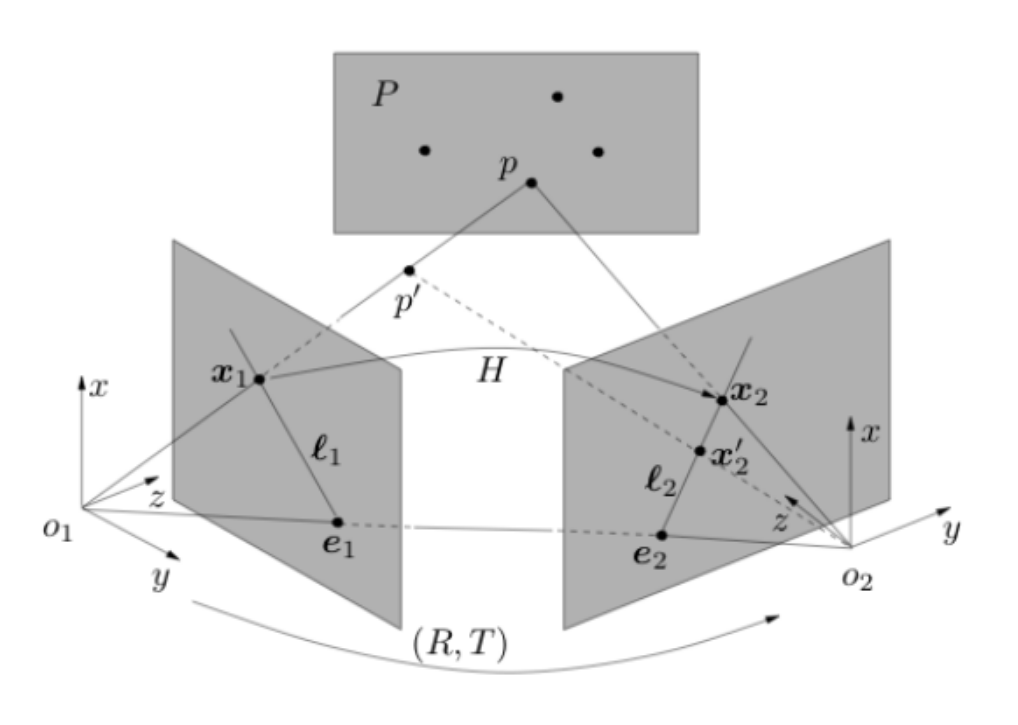
\includegraphics[width=0.6\linewidth]{image/Multiview-Geometry-Base/nonplanar_homography.png}  %插入的图,包括JPG,PNG,PDF,EPS等,放在源文件目录下
	\caption{非平面场景下的单应矩阵.}  %图片的名称
	\label{fig:nonplanar_homography}   %标签,用作引用
\end{figure}



\section{各种矩阵计算}






单应矩阵,DLT
基础矩阵,8点法,7点法
本质矩阵,8点法,5点法

\section{位姿计算}
\subsection{2D-2D}
本质矩阵分解
单应矩阵分解
\subsection{2D-3D}
PnP
\subsection{3D-3D}
3D-3D变换

\section{三角测量}



\chapter{Vocabulary Tree}
\section{Bag-of-Words模型简介}
解释清楚什么是视觉词汇
\section{TF-IDF}
解释清楚TF-IDF中IDF的含义


\section{DBoW2}
\subsection{TemplateVocabulary}
\begin{figure}[h]%%图
	\centering  %插入的图片居中表示
	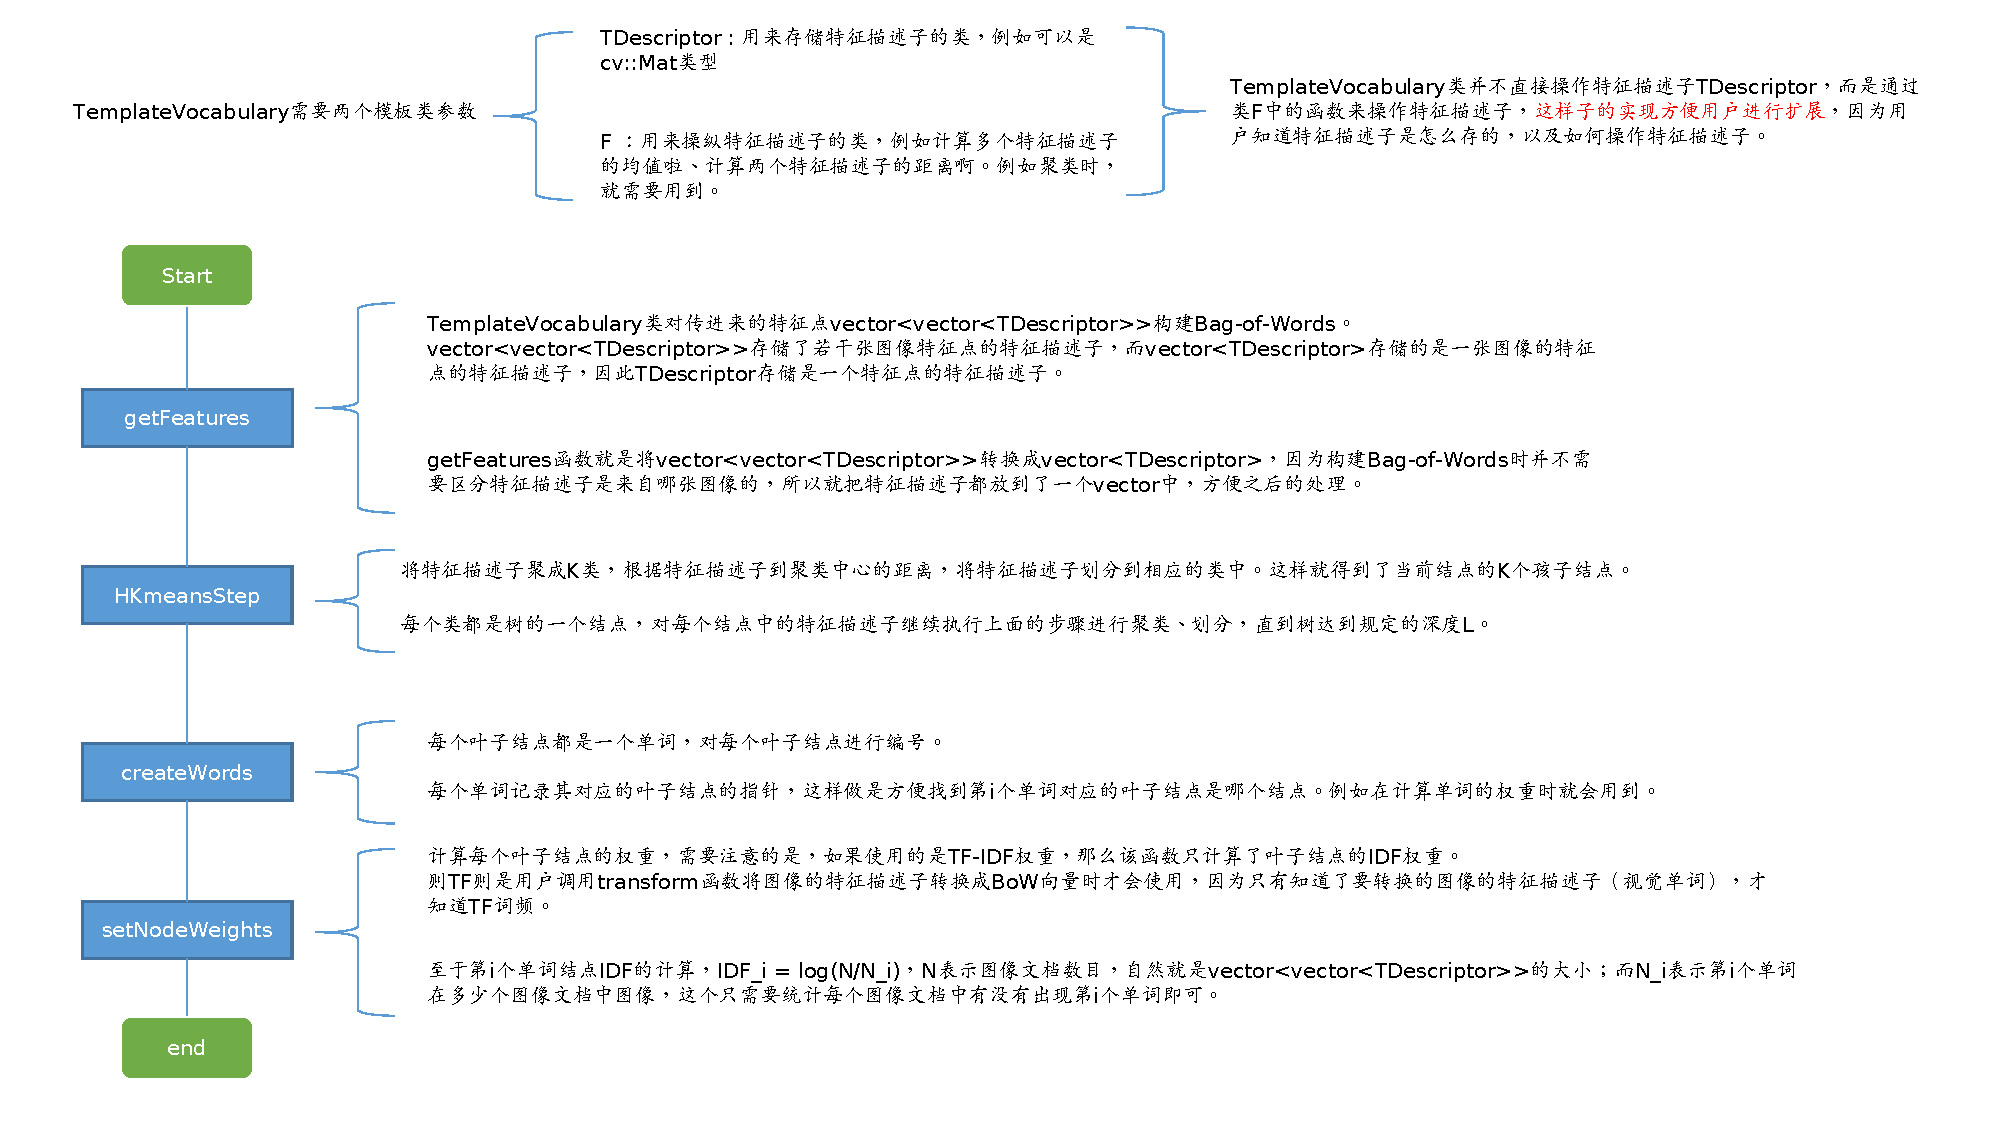
\includegraphics[width=1.0\linewidth]{image/DBoW2/DBoW2.pdf}  %插入的图,包括JPG,PNG,PDF,EPS等,放在源文件目录下
	\caption{词汇树构建流程.}  %图片的名称
\end{figure}


\subsection{BowVector}
建立完词汇树之后,可以将图像(特征描述子)转成BowVector表示,通过表示两个BoWVector的相似性从而得到两张图像的相似性,又因为比较两个BoWVector的速度很快,所以判断两张图片是否相似也就很快了。

构建完词汇树后,用户可以调用TemplateVocabulary的transform函数将图像转换成BoWVector表示(transform函数接受图像的特征描述子作为参数)。由于一般图像只有\textbf{几百}到\textbf{几千}个特征描述子,而词汇树种的叶子结点有\textbf{几百万}到\textbf{几千万}个,所以图像的BoWVector是稀疏向量,所以若直接用向量形式来表示,那么非常浪费空间,效率也不高。所以DBoW2使用STL中的map容器来存储这个向量。map容器中的key表示单词的id,而value则表示该单词的权重,该单词的权重为TF-IDF,其中TF为该单词在图像中出现的频率,而IDF则建树时,叶子结点根据训练集计算得到的权重。

将图像转为BoWVector表示之后,图像之间的相似性就表现为两个BoWVector的相似性。一般来说,图像的BoWVector都经过了L1范数归一化,并且计算相似性时也是使用两个BoWVector之间的L1范数。由于两个经过L1规范化的向量$v$和$w$差的L1范数$||v-w||_1$的范围在[0,2]之间,所以乘以一个$\frac{1}{2}$将其变到[0,1]之间。又因为我们想要L1范数越大表示两张图像越相似,所以将其变成$1 - \frac{1}{2}||v - w||_1$。

计算两个BoWVector之间的L1范数的公式如下:
\begin{eqnarray}
	||v - w||_1 = \sum_i^n |v_i - w_i|
\end{eqnarray}

由于BoWVector$v$和$w$是稀疏向量,上面的计算公式效率太低了,因此要对其进行优化。

对于$v_i$不为0且$w_i$不为0的情况,我们仍旧采用上面的公式进行计算:
\begin{equation}
	||v - w||_1 = \sum_i^n |v_i - w_i| \ , \ for \ all \ i \ and \ v_i \ne 0 \ and \ w_i \ne 0
\end{equation}


对于$v_i$不为0但$w_i$为0的情况:

\begin{equation}
\begin{split}
& ||v = w||_1  = \sum_i^n |v_i - w_i| = \sum_i^n |v_i| \ , \ for \ all \ i \ and \ v_i \ne 0 \ and \ w_i = 0 \\
& = 1 -  \sum_i^n |v_i|, for \ all \ i \ and \ v_i \ne 0 
\end{split}
\end{equation}


同理,对于$v_i$为0但$w_i$不为0的情况:

\begin{equation}
\begin{split}
& ||v = w||_1  = \sum_i^n |v_i - w_i| = \sum_i^n |w_i| \ ,\ for \ all \ i \ and \ v_i = 0 \ and \ w_i \ne 0 \\
& = 1 -  \sum_i^n |w_i| \ , for \ all \ i \ and \ w_i \ne 0 
\end{split}
\end{equation}

综上,得到:
\begin{equation}
	||v - w||_1 = 2 + \sum_i^n |v_i - w_i| -|v_i| - |w_i|  \ ,\ for \ all \ i \ and \ v_i \ne 0 \ and \ w_i \ne 0 \\
\end{equation}



所以,在计算两个BoWVector的相似性时,由于BoWVector使用STL的map进行存储,map容器中的key表示单词的id,而value则表示该单词的权重。所以只需要找到两个map中key相同的元素,进行上面的计算即可。实际的代码如下:

\begin{lstlisting}[language = C++]
double L1Scoring::score(const BowVector &v1, const BowVector &v2) const
{
	BowVector::const_iterator v1_it, v2_it;
	// 得到两个BoW向量的迭代器,实际上是map容器的迭代器
	const BowVector::const_iterator v1_end = v1.end();
	const BowVector::const_iterator v2_end = v2.end();
	
	v1_it = v1.begin();
	v2_it = v2.begin();
	
	double score = 0;
	
	while(v1_it != v1_end && v2_it != v2_end)
	{
		const WordValue& vi = v1_it->second;
		const WordValue& wi = v2_it->second;
		
		// 当两个BoW向量中,相同单词的权重都不为空时,根据公式进行计算
		if(v1_it->first == v2_it->first)
		{
			score += fabs(vi - wi) - fabs(vi) - fabs(wi);
			
			// move v1 and v2 forward
			++v1_it;
			++v2_it;
		}
		else if(v1_it->first < v2_it->first)
		{
			// move v1 forward
			v1_it = v1.lower_bound(v2_it->first);
			// v1_it = (first element >= v2_it.id)
		}
		else
		{
			// move v2 forward
			v2_it = v2.lower_bound(v1_it->first);
			// v2_it = (first element >= v1_it.id)
		}
	}
	
	// ||v - w||_{L1} = 2 + Sum(|v_i - w_i| - |v_i| - |w_i|) 
	//		for all i | v_i != 0 and w_i != 0 
	// (Nister, 2006)
	// scaled_||v - w||_{L1} = 1 - 0.5 * ||v - w||_{L1}
	score = -score/2.0;
	
	return score; // [0..1]
}


\end{lstlisting}


\subsection{FeatureVector}
我们知道闭环检测时,需要知道找到与当前关键帧相似的图像帧,
BowVector的作用在于快速判断两张图像的相似性;在找到相似的图像之后,需要做的就是找到两张图像中特征点的匹配关系,这当然可以使用KDTree来办到,但是这太慢了(要先对一张图像的特征点构建KDTree,另一张图像才能使用特征点进行查询),DBoW2的作者使用FeatureVector来实现快速找到两张图像中特征点的匹配关系。


我们知道图像的每个特征点对应了哪个叶子结点,那么也就知道了哪个叶子结点id对应了哪个特征描述子,所以类似BowVector的原理,对于FeatureVector也使用STL的map进行存储,其中key表示叶子结点的id,value表示经过该叶子结点的特征描述子(的id),那么接下来的比较就是类似BoW向量的比较,只需要比较两个FeatureVector(两个map)中具有相同叶子结点id的那些特征描述子。由于不同的特征描述子可能经过同一个叶子结点,所以FeatureVector的实际结构是这样的:FeatureVector类继承了std::map<int, std::vector<unsigned int>>类,其中key表示结点的id(不一定是叶子结点id),std::vector<unsigned int>表示经过该结点的特征描述子都有哪些。

之前不是说map的key表示叶子结点的id,那么为什么现在又说key表示的不一定是叶子结点的id呢?这是为了提高特征匹配的正确性,
由于词汇树可能划分地太细了,可能导致两个相似的特征描述子被分在了两个相邻的叶子结点上,若是我们只要相同的叶子结点上进行特征描述子的比较,那么就会错过正确的匹配。但是我们发现,虽然它们被分在了相邻的叶子结点,但是它们经过了同一个父亲结点啊,由于词汇树的特性,两个特征描述子只要经过了相同的结点,那么其就有可能是正确的匹配。为了提高鲁棒性,现在FeatureVector的map中的key存储的不再是叶子结点的id(倒数第一层结点的id),可能是倒数第二层、第三层结点的id(ORB-SLAM2使用的是倒数第四层的,可能是经过了一些测试采用的吧),而value则表示经过那些结点的特征描述子有哪些。至于比较过程,还是只需比较具有相同结点id的那些特征描述子即可。


\subsection{TemplateDatabase}
如果我们想在n张图像中找到与查询图像相似的图像该怎么办?如果使用TemplateVocabulary,那么就是讲n张图像和查询图像转换成BoWVector表示,然后对于n张图像中的每张图像和查询图像之间利用BoWVector计算相似性,然后按照相似性,找到相似图像。


TemplateDatabase的作用就是用来快速在一堆图像中找到与查询图像相似的图像的。

构造TemplateDatabase时,需要传入一个词汇树(构造好的TemplateVocabulary对象);然后需要不断调用add函数,将图像的特征描述子添加到TemplateDatabase中,该函数构建了图像的invert list,也即记录了每个叶子结点都被哪张图像的特征描述子经过。

在查询时,只需要遍历查询图像的BoWVector,然后通过invert list累积相应图像的评分,最终哪张图像的评分最高,那么哪张图像就与查询图像最相似。



\section{参考文献}
DBoW2算法原理 http://www.cnblogs.com/jian-li/p/5664559.html


\chapter{SLAM基础}
\section{闭环检测}
没有闭环检测的SLAM系统叫做视觉里程计(VO),视觉里程计随着时间的推移,误差会随之累计,从而导致位姿误差累计,从而导致3D点位置的不正确,从而导致在闭环处,本应该相同的3D场景点,被重建到了不同的3D点,并且离得还挺远的,从而导致了漂移。如下图所示:

\begin{figure}[h]%%图
	\centering  %插入的图片居中表示
	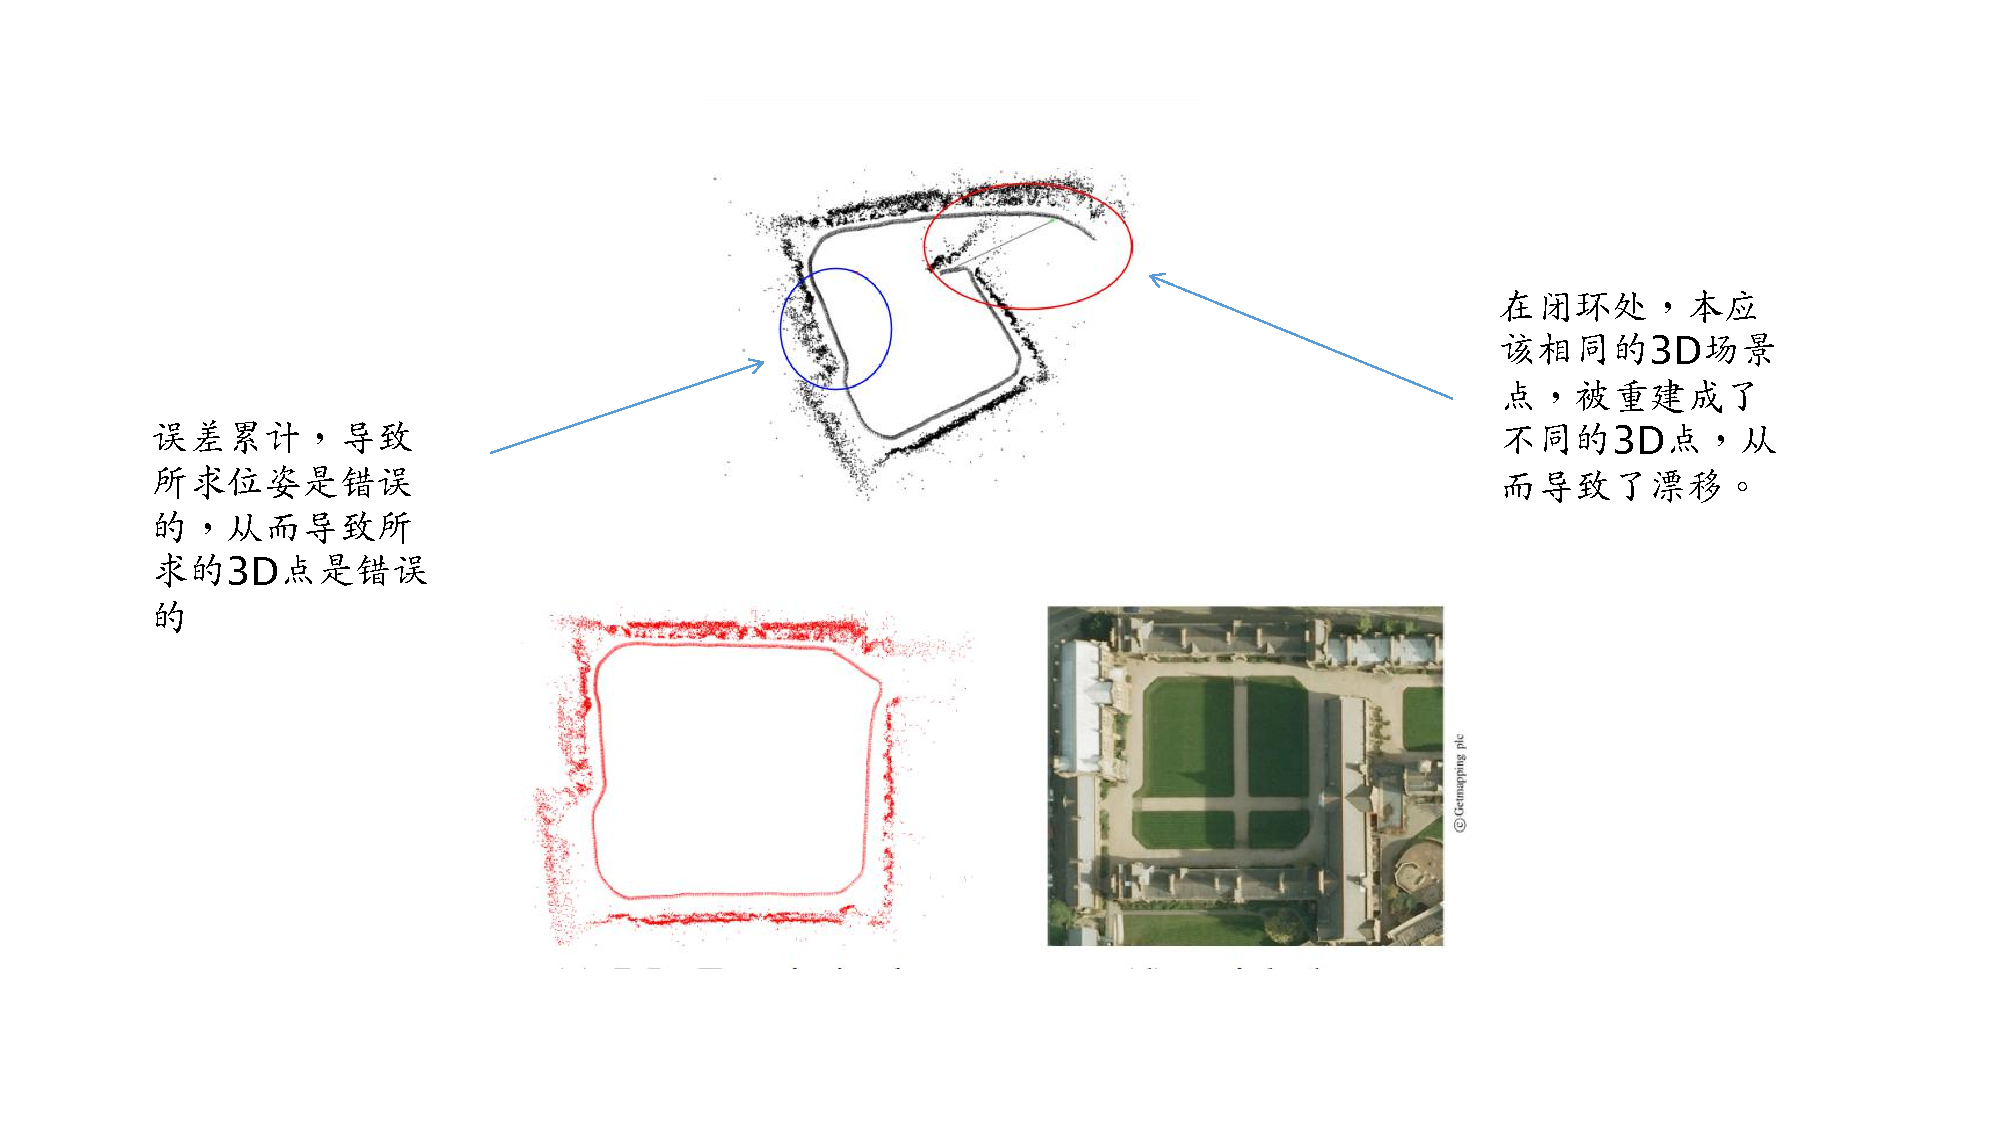
\includegraphics[width=1.0\linewidth]{image/drift.pdf}  %插入的图,包括JPG,PNG,PDF,EPS等,放在源文件目录下
	\caption{3D点误差累积及漂移.}  %图片的名称
	\label{fig:tracking}   %标签,用作引用
\end{figure}


相机的位姿不准(累积误差),从而导致3D点的位置不准,在闭环处就表现为:\textbf{本应该重合的3D点,因为位姿不准,而不重合了,漂移了},我能理解漂移,但是不能够理解\textbf{尺度漂移}。

而\textbf{闭环纠正},就是使用很久之前很久之前的相机位姿(准)重新计算闭环的相机位姿(不准->准),从而减少了累积误差,但是这里的重新计算只是纠正了闭环帧的累积误差,为了进一步减少其它帧的累积误差,我们需要将结果传播出去,具体表示为pose graph优化,但是pose graph优化又认为相对位姿是准的,这就令我很不明白了。




\textbf{pose graph的约束都是如何得到的}:
\begin{enumerate}
	\item 相邻关键帧之间的位姿约束
	\item 时间序列上比较接近的关键帧之间的位姿约束(可以称作局部回环),比如t时刻的关键帧不仅仅与t-1时刻的关键帧构成约束关系,还会与t-2时刻的关键帧构成约束关系。
	\item  时间序列上不接近,而空间上接近的关键帧之间的位状约束(可以称作大回环),一般来说,机器人绕着房子周围走了一圈回到了起点,那么检测到的回环就是大回环。
\end{enumerate}





\section{Pose Graph和闭环检测}
带有相机位姿和空间点的图优化称为 BA,能够有效地求解大规模的定位与建图问题。BA能够有效解决漂移(从我实现SFM系统的经验可得),但是由于BA数据量太大了,不适合需要实时性的SLAM。适合SLAM优化的解决方案有两种,一种是移动窗口BA;另一种就是Pose Graph。
	
Pose Graph就是将相机的绝对位姿作为图的结点(待优化变量),而相机之间的相对位姿作为边(约束条件),当遇到回环时,通过位姿图进行优化,就能够减少累计误差。

\begin{note}
	不是很理解位姿图优化,不会将位姿优化飘掉吗?
\end{note}
	
使用frame-to-frame的方式求得的位姿,会使得误差逐渐累积,从而导致位姿越来越不准。因为后一帧图像的位姿是基于前一帧图像进行计算的,如果前一帧图像的位姿具有误差,哪怕很小,那么后一帧图像计算得到的位姿也会使得误差增加。随着SLAM系统的不断运行,这个误差就越来越大,从而导致相机都轨迹都出现了漂移。

\begin{figure}[h]%%图
	\centering  %插入的图片居中表示
	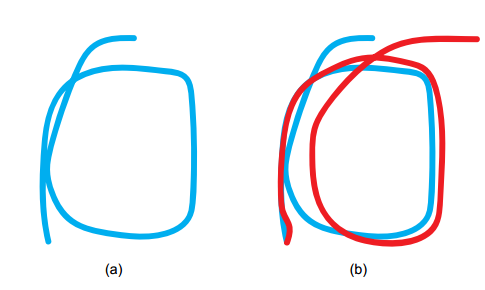
\includegraphics[width=0.7\linewidth]{image/Trajectory_drift}  %插入的图,包括JPG,PNG,PDF,EPS等,放在源文件目录下
	\caption{漂移示意图。( a)真实轨迹;( b)漂移轨迹.}  %图片的名称
	\label{fig:Trajectory_drift}   %标签,用作引用
\end{figure}
	
虽然随着SLAM系统的运行,相机的绝对位姿的误差会越来越大,但是相邻两关键帧之间的位姿还是挺准确的,所以每个关键帧和其前续(predecessor)关键帧之间的相对位姿可以构成一个约束。

\begin{note}
	相邻关键帧的位姿态就一定准确吗?对于RGB-D相机,计算相邻关键帧的位姿时,使用的3D点是从相机得到的,那么计算得到的相邻位姿应该是准确的;但是对于RGB相机,使用的3D点就是具有累计误差的,那么使用该3D点计算得到的相邻位姿应该不能认为是准确的吧。
\end{note}



\chapter{LSD SLAM}
\section{程序流程}

整个程序大致有4个线程(一些能够并行的任务也用来了线程池来计算):

分别是主线程用来追踪每一帧的位姿,并决定是否创建关键帧,流程如图\ref{fig:tracking}所示;

mappingThreadLoop线程,用来构建新的深度图或者是更新当前关键帧的深度图,流程如图\ref{fig:mapping_thread}所示;

constraintSearchThreadLoop线程,用来除当前关键帧之外的那些关键帧是否存在闭环,如果存在闭环,则生成pose graph的约束关系,并插入到pose graph中,流程如图\ref{fig:constraint_search_thread}所示;

optimizationThreadLoop线程,用来对已经构建的位姿图进行优化,流程如图\ref{fig:mapping_thread}所示。


\begin{figure}[h]%%图
	\centering  %插入的图片居中表示
	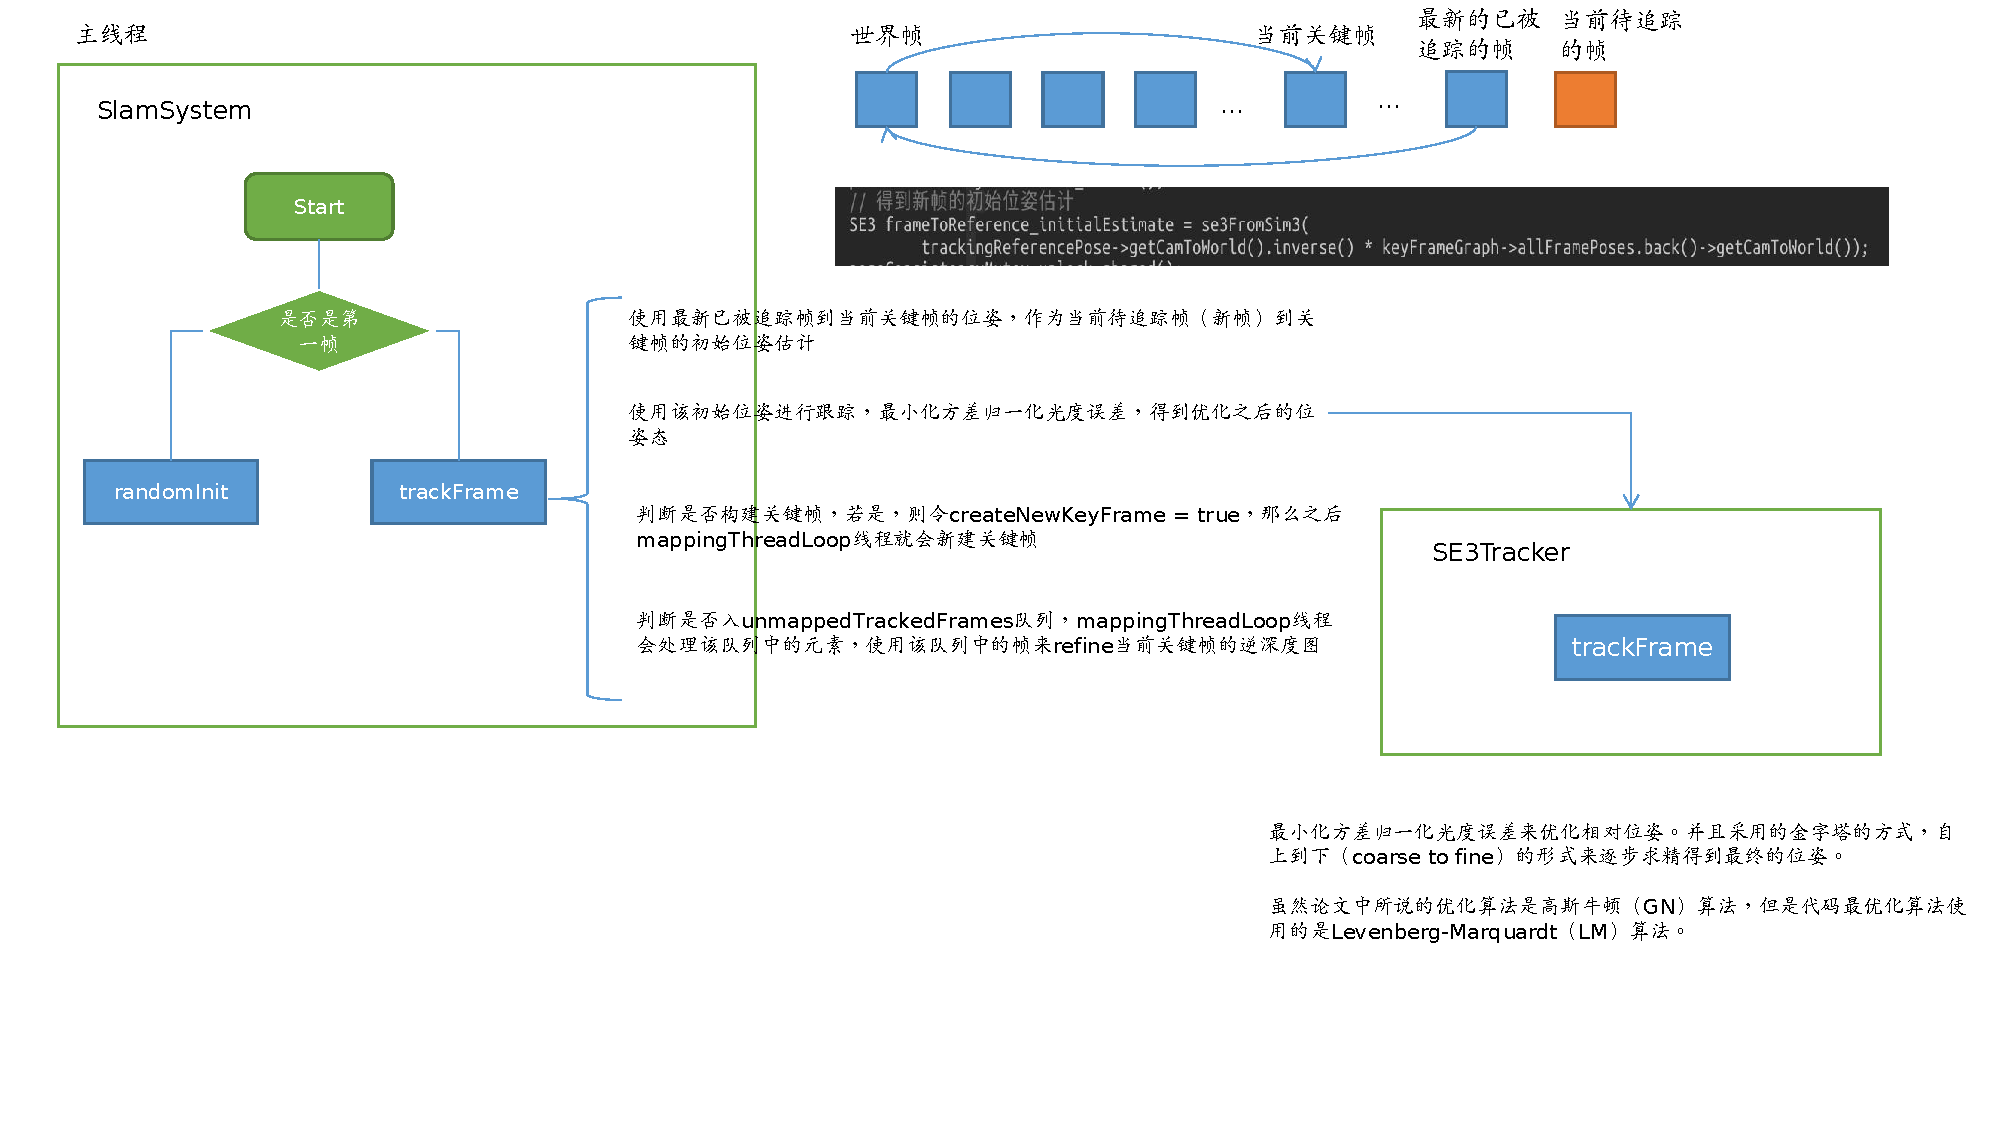
\includegraphics[width=1.0\linewidth]{image/LSD-SLAM/LSD-SLAM-tracking.pdf}  %插入的图,包括JPG,PNG,PDF,EPS等,放在源文件目录下
	\caption{跟踪流程图.}  %图片的名称
	\label{fig:tracking}   %标签,用作引用
\end{figure}





\begin{figure}[h]%%图
	\centering  %插入的图片居中表示
	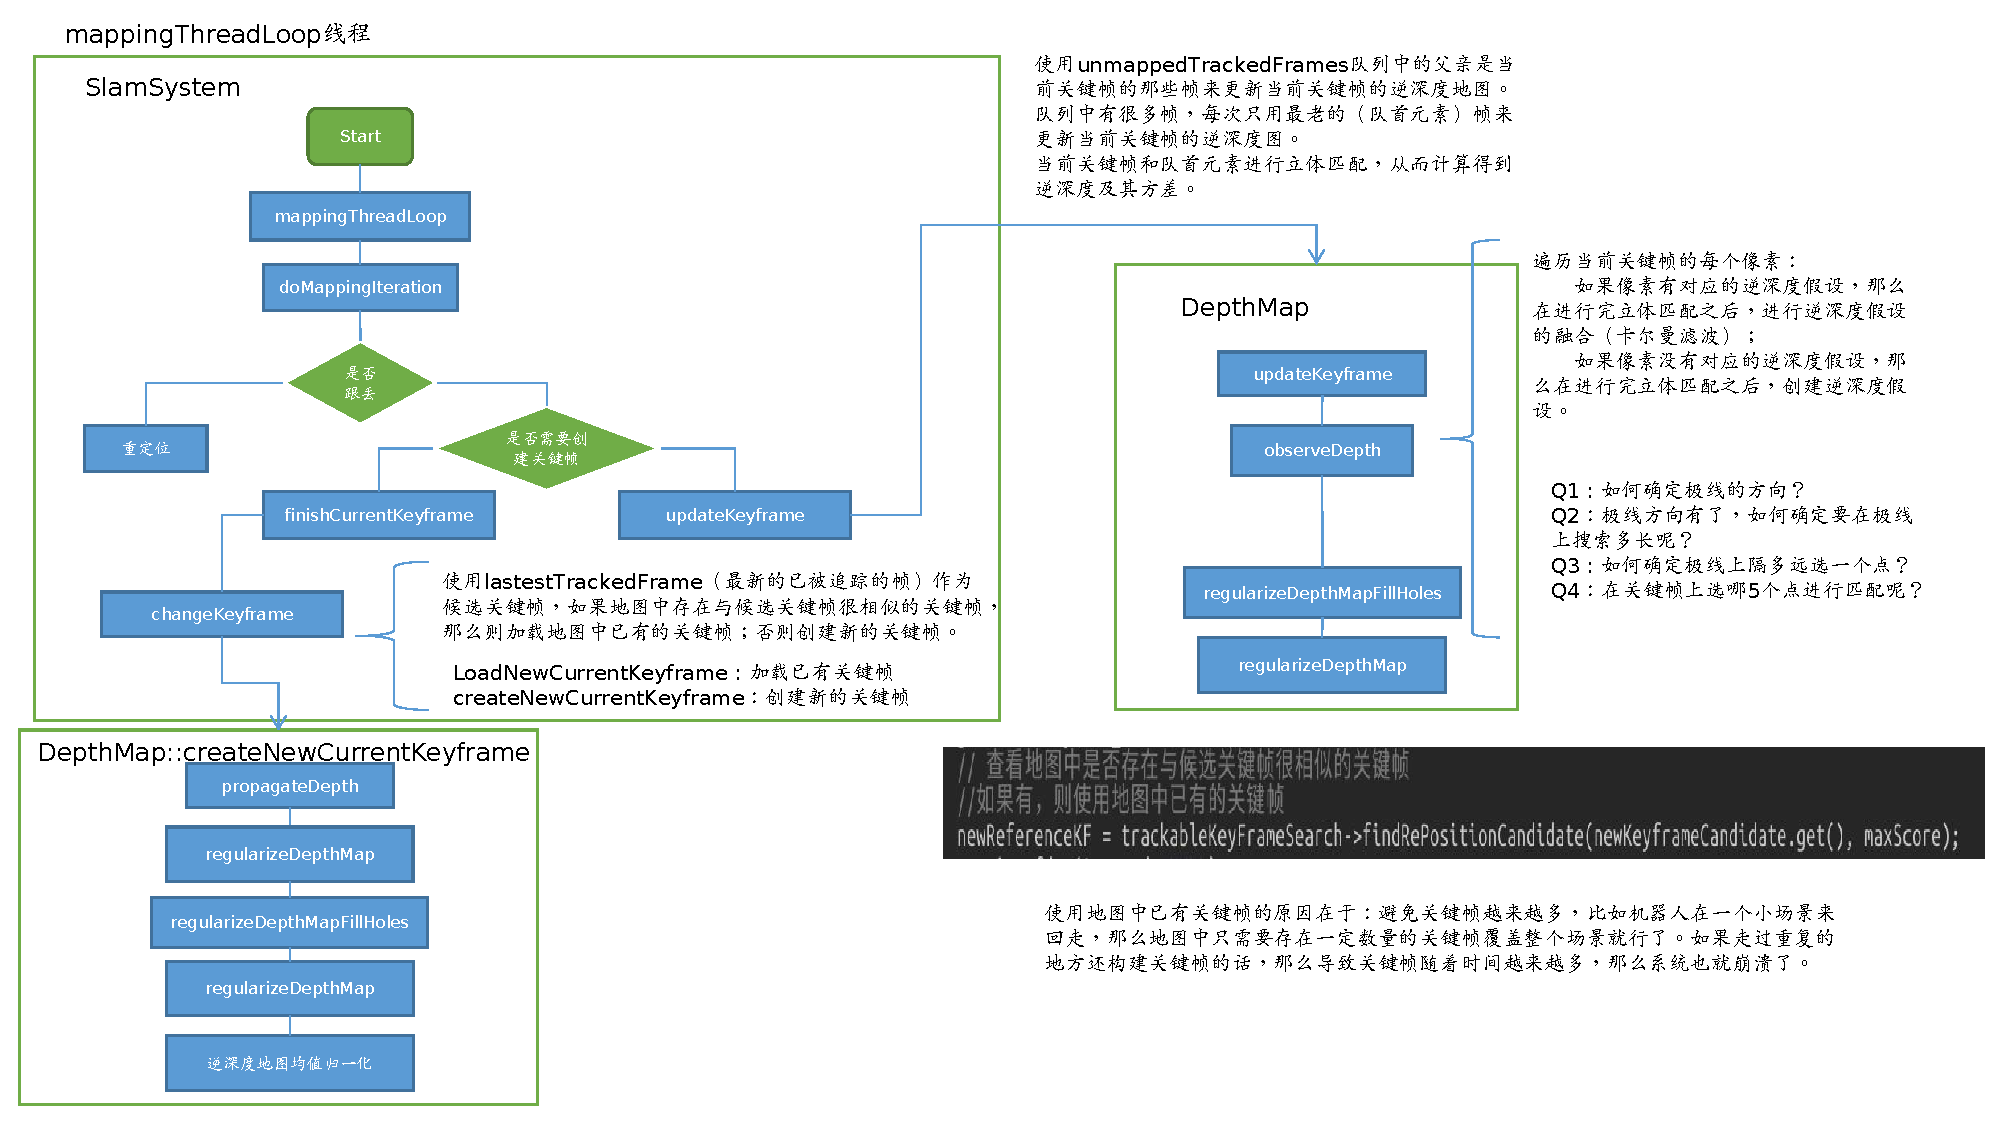
\includegraphics[width=1.0\linewidth]{image/LSD-SLAM/LSD-SLAM-mapping}  %插入的图,包括JPG,PNG,PDF,EPS等,放在源文件目录下
	\caption{mappingThreadLoop流程图.}  %图片的名称
	\label{fig:mapping_thread}   %标签,用作引用
\end{figure}



\section{Tracking}
\subsection{公式推导}
\subsubsection{归一化光度误差}
	LSD SLAM的帧间追踪,也是基于直接法的一般套路,使用前一帧到参考帧的相对位姿作为参考帧到当前帧相对位姿的初始估计(基于小运动假设),然后通过最小化光度误差(photometric error)来得到优化过后的位姿态。
	
	不过,LSD SLAM在一般光度误差的基于上进行了改善,使用的是方差归一化光度误差(variance-normalized photometric error)
\begin{equation}
E_p(\bm{\xi}_{ji}) = \sum_{p \in \Omega_{D_i}}\| \frac{r_p^2(\bm{p}, \bm{\xi}_{ji})}{\sigma_{r_p}^{2}(\bm{p}, \bm{\xi}_{ji})} \|_\delta
\end{equation}

其中
\begin{equation}
	r_p(\bm{p},\bm{\xi}_{ji}) := I_i(\bm{p}) - I_j(\omega(\bm{p}, D_i(\bm{p}), \bm{\xi}_{ji}))
\end{equation}

\begin{equation}
	\sigma_{r_p}^{2}(\bm{p}, \bm{\xi}_{ji}) := 2\sigma_I^2 + (\frac{\partial r_p(\bm{p}, \bm{\xi}_{ji})}{\partial D_i(\bm{p})})^2V_i(\bm{p})
\end{equation}

这里的$||*||_\delta$为Huber-norm,表示为:
\begin{equation}
	||r^2||_\delta := 
		\begin{cases}
			\frac{r^2}{2\delta} &  if \ \ |r| \le \delta \\
			|r| - \frac{\delta}{2} & otherwise\\
		\end{cases}
\end{equation}

式子中的$\bm{\xi}_{ji}$就是要求得两帧之间的SE3变换(从$i \rightarrow j$,也就是参考帧到当前帧的变换),这里使用李代数的形式表示;这里的$\bm{p}$是在参考帧$I_i$下观测到的有深度信息($\bm{p} \in \Omega_{D_i}$)的\textbf{归一化相机平面上的点};函数$D_i(\bm{p})$是点$p$在参考帧下的\textbf{逆深度},$V_i(\bm{p})$是对应的逆深度的方差;函数$\omega(\bm{p}, D_i(\bm{p}), \bm{\xi}_{ji})$则是将参考帧下的图像像素坐标根据逆深度反向投影得到3D点,然后将3D点投影到当前帧的图像平面;这里的$\sigma_I^2$是图像的高斯噪声。

\begin{note}
	以上公式都省略了相机内参,也即省略了归一化相机平面坐标到图像像素平面坐标的转换($ \bm{u} = \bm{K}\bm{p}$),但是在LSD SLAM的代码中是不会省略的。
\end{note}


论文在计算两帧之间位姿变换时,将所有有逆深度假设的像素都用上了。但是每个逆深度的确定性不同,也就是有些逆深度比较准确(方差$V_i(\bm{p})$小),有些不准确(方差$V_i(\bm{p})$大)。因此在公式(1.1)中在残差上除以方差做了归一化。方差的第一项是两个图像的高斯噪声,第二项则是使用了方差传播公式计算得到的,即由于误差是使用\textbf{逆深度}计算得到的,那么逆深度的方差就会传播到误差的方差。所以将光度误差除以其方差,就得到了方差归一化的光度误差,这里应该是利用了马氏距离的思想。


公式(1.1)、(1.2)、(1.3)、(1.4)就是LSD计算位姿时,所使用的误差函数,公式中的大部分都比较简单,且在其它SLAM都有的东西,主要是公式(1.3)中误差中\textbf{逆深度}的求导是比较新的东西,下面对其导数进行推导:


%\begin{align*}
%	&\frac{\partial [I_i(\bm{p}) - I_j(\omega(\bm{p}, D_i(\bm{p}), \bm{\xi}_{ji}))]}{\partial D_i(\bm{p})} \\
%	&= - \frac{\partial I_j(\omega(\bm{p}, D_i(\bm{p}), \bm{\xi}_{ji}))}{\partial D_i(\bm{p})} \\
%	&= -\frac{\partial I_j(\bm{u}')}{\partial \bm{u}'} \frac{\partial \bm{u}'}{\partial \bm{p}'} \frac{\partial \bm{p}'}{\partial \bm{X}'} \frac{\partial \bm{X}'}{\partial D_i(\bm{p})}
%\end{align*}


首先,列出一些必要的公式
\begin{equation}
\bm{u} = \bm{K} \bm{p}
\end{equation}

\begin{equation}
\bm{u}' = \bm{K} \bm{p}'
\end{equation}

\begin{equation}
\bm{X} = \frac{1}{D_i(\bm{p})} \bm{p} =  \frac{1}{D_i(\bm{p})} \bm{K}^{-1} \bm{u}
\end{equation}

\begin{equation}
\bm{X}' = R \frac{1}{D_i(\bm{p})} \bm{K}^{-1} \bm{u} + t
\end{equation}


其中$\bm{u}'$是参考帧图像$I_i$的像素平面坐标点$\bm{u}$在当前帧图像$I_j$下的对应点;$\bm{X}'$则是点$\bm{u}'$在当前帧相机坐标系下所对应的3D点,该3D点是参考帧图像$I_i$的归一化平面点$\bm{p}$根据逆深度$D_i(\bm{p})$反向投影,然后根据位姿$\bm{\xi}_{ji}$旋转平移得到的.


那么根据链式法则,能够得到下面的导数:


\begin{equation}
	\begin{split}
		&\frac{\partial [I_i(\bm{p}) - I_j(\omega(\bm{p}, D_i(\bm{p}), \bm{\xi}_{ji}))]}{\partial D_i(\bm{p})} \\
		&= - \frac{\partial I_j(\omega(\bm{p}, D_i(\bm{p}), \bm{\xi}_{ji}))}{\partial D_i(\bm{p})} \\
		&= -\frac{\partial I_j(\bm{u}')}{\partial \bm{u}'} \frac{\partial \bm{u}'}{\partial \bm{X}'}  \frac{\partial \bm{X}'}{\partial D_i(\bm{p})}
	\end{split}
\end{equation}







导数的第一项是图像梯度:
\begin{equation}
\frac{\partial I_j(\bm{u}')}{\partial \bm{u}'} = 
	\left[
	\begin{array}{cc}
		gx & gy
	\end{array}
	\right]
\end{equation}

根据公式(1.7)知道$\bm{X}'$是如何计算得到$\bm{u}'$的,从而得到导数的第二项如公式(1.8)所示:

\begin{equation}
	\bm{u}' = \left[ \begin{array}{c}
		u' \\
		v'
	\end{array}\right] 
	= \frac{1}{Z'}  
		\left[ \begin{array}{ccc}
			fx & 0 & cx \\
			 0 & fy& cy \\
			 0 & 0 & 1 
		\end{array}\right]
		\left[ \begin{array}{c}
			X' \\
			Y' \\
			Z' 
		\end{array}
		\right]
	= \left[ \begin{array}{c}
		(fx X' + cx) / Z' \\
		(fy Y' + cy) / Z' \\
	\end{array}\right]
\end{equation}


\begin{equation}
	\frac{\partial \bm{u}'}{\partial \bm{X}'}
	=
	\left[ 
		\begin{array}{ccc}
			\frac{fx}{Z'} & 0 & -\frac{fxX'}{Z'^2} \\
			0 & \frac{fy}{Z'} & -\frac{fyY'}{Z'^2} 
		\end{array}
	\right]
\end{equation}


根据公式(1.9)知道$\bm{X}'$是如何根据$\bm{p}$、逆深度$D_i(\bm{p})$以及位姿$\bm{\xi}_{ji}$计算得到的,所以导数的第三项如公式(1.10)所示:


\begin{equation}
	\frac{\partial \bm{X}'}{\partial D_i(\bm{p})}
	=
	-\frac{1}{D_i(\bm{p})^2}\bm{R}\bm{K}^{-1} \bm{u}
\end{equation}

进行进一步推导,能够得到:

\begin{equation}
	\bm{X}' = \frac{1}{D_i(\bm{p})} \bm{R} \bm{K}^{-1}\bm{u} + \bm{t}
\end{equation}
\begin{equation}
	-\bm{X}' = -\frac{1}{D_i(\bm{p})} \bm{R} \bm{K}^{-1}\bm{u} - \bm{t}
\end{equation}
\begin{equation}
	\bm{t} -\bm{X}' = -\frac{1}{D_i(\bm{p})} \bm{R} \bm{K}^{-1}\bm{u}
\end{equation}

\begin{equation}
\frac{\bm{t} -\bm{X}'}{D_i(\bm{p})} = -\frac{1}{D_i(\bm{p})^2} \bm{R} \bm{K}^{-1}\bm{u}
\end{equation}
\begin{equation}
		\frac{\partial \bm{X}'}{\partial D_i(\bm{p})} = \frac{\bm{t} -\bm{X}'}{D_i(\bm{p})}
		= 
		\frac{1}{D_i(\bm{p})}
		\left[
			\begin{array}{c}
				t_x - X' \\
				t_y - Y' \\
				t_z - Z'
			\end{array}
		\right]
\end{equation}



综上所述,得到最终的导数是:
\begin{equation}
\begin{split}
	&-\left[
		\begin{array}{cc}
			gx & gy
		\end{array}
	\right]
	\left[ 
		\begin{array}{ccc}
			\frac{fx}{Z'} & 0 & -\frac{fxX'}{Z'^2} \\
			0 & \frac{fy}{Z'} & -\frac{fyY'}{Z'^2} 
		\end{array}
	\right]		
	\frac{1}{D_i(\bm{p})}
	\left[
		\begin{array}{c}
			t_x - X' \\
			t_y - Y' \\
			t_z - Z'
		\end{array}
	\right] \\
	&=
	-\left[
		\begin{array}{cc}
			gx fx &	gy fy
		\end{array} 
	\right]
	\left[ 
		\begin{array}{c}
			\frac{t_x - X'}{Z'D_i(\bm{p})^2}- \frac{(t_z - Z')X'}{Z'^2 D_i(\bm{p})}\\
			\frac{t_y - Y'}{Z'D_i(\bm{p})^2}- \frac{(t_z - Z')Y'}{Z'^2 D_i(\bm{p})}\\
		\end{array}
	\right]
\end{split}
\end{equation}


通分,整理合并之后,得到LSD SLAM代码中误差光度误差关于逆深度$D_i(\bm{p})$的导数为:

\begin{equation}
\begin{split}
&\frac{\partial [I_i(\bm{p}) - I_j(\omega(\bm{p}, D_i(\bm{p}), \bm{\xi}_{ji}))]}{\partial D_i(\bm{p})} \\
&=
-\left[
\begin{array}{cc}
gx fx & gy fy
\end{array} 
\right]
\left[ 
\begin{array}{c}
\frac{txZ' - tzX'}{Z'^2D_i(\bm{p})}\\
\frac{tyZ' - tzY'}{Z'^2D_i(\bm{p})}\\
\end{array} 
\right]
\end{split}
\end{equation}




参考 : \href{https://zhuanlan.zhihu.com/p/54129298}{LSD-SLAM权重更新公式推导}




\subsubsection{加权最小二乘法}


\begin{equation}
E_p(\bm{\xi}_{ji}) = \sum_{p \in \Omega_{D_i}}\| I_i(\bm{p}) - I_j(\omega(\bm{p}, D_i(\bm{p}), \bm{\xi}_{ji}))  \|^2
\end{equation}

\begin{equation}
	\min_{\bm{\xi}_{ji}} E_p(\bm{\xi}_{ji})
\end{equation}
普通最小二乘法就是直接最小化该误差,从而得到优化过有的位姿。由附录\ref{appendix:non-linear-least-square}可得该非线性最小二乘的解如下:
\begin{equation}
	\delta \bm{\xi}_{ji}^{(n)} = -(J^TJ)^{-1} J^Tr(\bm{\xi}_{ji}^{(n)})
\end{equation}

位姿的更新公式为:
\begin{equation}
	\bm{\xi}_{ji}^{(n+1)} = \delta \bm{\xi}_{ji}^{(n)} \circ \bm{\xi}_{ji}^{(n)}
\end{equation}




为了减少外点的影响,例如由于遮挡(occlusions)和镜面反射(reflections)所导致的错误的点对应,作者使用了加权最小二乘,在每次迭代时,计算权重$\bm{W}=\bm{W}(\bm{\xi}_{ji}^{(n)})$。
所以误差函数变为:
\begin{equation}
	E_p(\bm{\xi}_{ji}) = \sum_{p \in \Omega_{D_i}} w_p(\bm{\xi}_{ji}) \| I_i(\bm{p}) - I_j(\omega(\bm{p}, D_i(\bm{p}), \bm{\xi}_{ji}))  \|^2
\end{equation}
从而最小二乘的解变为:
\begin{equation}
		\delta \bm{\xi}_{ji}^{(n)} = -(J^TWJ)^{-1} J^TWr(\bm{\xi}_{ji}^{(n)})
\end{equation}

该权重就是误差的方差的倒数,并经过Huber-norm进行加权,也即公式(1.3)与公式(1.4)。
需要注意的是,在代码的实现中误差并没有经过Huber-norm进行加权。这与公式(1.1)不符。

\subsection{代码解析}




LSD SLAM通过最小化方差归一化光度误差来求解两帧图像之间的位姿变化,并且采用了LM算法迭代求解。LSD SLAM求解两帧图像的SE3变换的函数主要在\textbf{SE3Tracker}中实现中。该类中有四个函数比较重要,分别为

\begin{itemize}
	\item \href{https://github.com/tum-vision/lsd_slam/blob/catkin/lsd_slam_core/src/Tracking/SE3Tracker.cpp#L280}{SE3Tracker::trackFrame}
	\item \href{https://github.com/tum-vision/lsd_slam/blob/catkin/lsd_slam_core/src/Tracking/SE3Tracker.cpp#L885}{SE3Tracker::calcResidualAndBuffer}
	\item \href{https://github.com/tum-vision/lsd_slam/blob/catkin/lsd_slam_core/src/Tracking/SE3Tracker.cpp#L749}{SE3Tracker::calcWeightsAndResidual}
	\item \href{https://github.com/tum-vision/lsd_slam/blob/catkin/lsd_slam_core/src/Tracking/SE3Tracker.cpp#L1277}{SE3Tracker::calculateWarpUpdate}
\end{itemize}


\begin{lstlisting}[language = C++]
SE3 SE3Tracker::trackFrame(
	TrackingReference* reference,
	Frame* frame,
	const SE3& frameToReference_initialEstimate);
\end{lstlisting}

函数\textbf{SE3Tracker::trackFrame}需要传入三个形参,从参考帧到当前帧,首先是两帧图像帧的实例,另外就是给定的两帧之间的\textbf{初始相对位姿},对于\textbf{初始相对位姿},LSD SLAM使用了上一帧到参考帧的位姿作为当前位姿估计的初始值。

\textbf{SE3Tracker::trackFrame}函数的主体是一个for循环,从金字塔的高层开始遍历知道底层。在循环内使用加权高斯牛顿法算法(Weighted Gauss-Newton Optimization)来对位姿进行优化,并使用金字塔上一层优化过后的位姿作为下一层的初始位姿。该函数的代码结构可以归纳如下:


\begin{lstlisting}
从上到下遍历金字塔的每一层
step1 : 对参考帧当前层构造点云(reference->makePointCloud)
step2 : 使用也有的位姿估计计算残差以及一些所需要的数据,并存放到buffer中(calcResidualAndBuffers)
step3 : 计算残差的权重,也即残差的方差的倒数(calcWeightAndResidual)
step4 : 计算每个残差的雅克比向量,并更新A和b(calculateWarpUpdate)
step5 : 计算得到增量inc = A.ldlt().solve(b)

\end{lstlisting}



在GN优化时,在每次迭代之后都要重新计算雅克比矩阵、残差以及权重矩阵。雅克比矩阵和残差在函数\textbf{SE3Tracker::calcResidualAndBuffers}中计算,而权重矩阵(实际上是权重系数)在\textbf{SE3Tracker::calcWeightAndResidual}中计算。接着在函数\textbf{SE3Tracker::calculateWarpUpdate}中构造方重组,最后求解方程组。


作者论文中说的是GN优化算法,但是代码中实际使用的是LM算法优化,LM算法的区别于GN算法的地方在于求解最小二乘$Ax=b$的时候,增加了一个系数$\lambda$,也就是$(A+\lambda I)x=b$。$\lambda$越大,越接近梯度下降法。 在代码中,如果此次迭代收敛(此次误差相对于前一次的误差减少了),那么减少$\lambda$的权重,如果此次迭代不收敛(此次误差相对于前一次的误差增大了),那么增大$\lambda$的权重。


更加详细的源码阅读,可以看这篇笔记:\href{https://www.zybuluo.com/kokerf/note/855220}{LSD-SLAM笔记之SE3Tracking};或者是这篇笔记:\href{https://www.baidu.com/link?url=gFb5QHUu2_4TmXHqie8m0oBYpXRHrJXFhlNW8pf9i-HOnoGS7nJXVs7YlJ88vmNC&wd=&eqid=f3e75ce0000ca6a5000000035c76477c}{LSD-SLAM解读——帧间追踪(详细推导)}


\section{DepthMap}
	
LSD SLAM构建的地图是半稠密逆深度地图(semi-dense inverse depth map),只对有明显梯度的像素位置进行深度估计,用逆深度表示,并且假设逆深度的噪声服从高斯分布。


\subsection{极线搜索的尺度问题}
LSD SLAM在当前关键帧上取5点,然后在参考帧上沿着极线移动,也取5点进行匹配。那么存在如下几个问题是需要想明白的:

\begin{enumerate}
	\item Q1 : 在关键帧上取哪5个点呢?
	\item Q2 : 在参考帧上,沿着极线取间隔多大的5个点呢?
	\item Q3 : 
\end{enumerate}



首先,我们分析一下二视图立体几何是如何计算视差图的。例如:对于左图中y = 5这行上的每个点x,只需要在右图中y = 5这行上进行极线搜索就行了。进一步进行分析,左图中y = 5这行上的每个点x,其在右图中的极线都是相同的,也即都是右图中y = 5这条直线;同理,右图中y = 5这行上的每个点x,其在左图中的极线也都是相同的,也即都是左图中y = 5这条直线。
\begin{note}
	这里应该有一张二视图视差搜索图。
\end{note}

将上面的结论推广到未进行极线矫正的两张图像上,左图中一条极线上的点,在右图中的极线都是相同的;同理,右图中一条极线上的点,在左图中的极线也是相同的。也就是说左图极线上的某些点,与右图极线上的某些点是匹配点。

所以,LSD SLAM对于在当前关键帧上的每个点$u$在参考帧上进行极线搜索时,是这么做的:

\begin{enumerate}
	\item 计算当前关键帧上的点$u$在参考帧上所对应的极线;
	\item 计算参考帧上的极线在当前关键帧上所对应的极线,由于过两点确定一条直线,在当前关键帧上对应的极线过点$u$和极点$e$
	\item 在当前关键帧上,在点$u$的附近按照极线方向,按照一定的距离,取5个点;
	\item  在参考帧上,沿着极线方向进行搜索,每次取间隔为单位长度1的5个点进行匹配。
	\item cost最小的点,就是匹配点。
\end{enumerate}


可能会有一个疑问就是,能够保证左图中过点$u$的极线只有一条吗。如果过点$u$的极线有多条,那么上面的方法算出来的极线可能不是我们想要的。这个担忧是没有必要的,\textbf{极线相交于极点,所以,对于非极点的像素点,其只会位于一条极线上,因为两条直线不可能相交于两点}。

\begin{note}
	如果点$u$和极点$e$非常接近,那么过点$u$的极线可能就不止一条了。这是因为所有的极线都过极点$e$,又因为$u$和极点$e$非常接近,所以导致过点$u$的极线可能不止一条了。所以说,如果点$u$和极点$e$非常接近时,根据上面的方法计算得到的极线方向可能是不稳定的,所以不能要。所以,LSD SLAM的代码中,也有对得到的极线长度的平方进行判断,如果太短了,小于1,那么就认为不稳定。
\end{note}



已知参考帧到当前关键帧的相对旋转和平移为$R$和$t$,也即默认参考帧为世界坐标系的情况下,参考帧的光心在当前关键帧下的坐标为:
\begin{equation}
	O = R \left[\begin{array}{c}
		0 \\
		0 \\
		0
	\end{array}\right] + t = t
\end{equation}

参考帧的光心在当前关键帧上的投影为
\begin{equation}
	e = KO = 
		\frac{1}{o_z}\left[ 
			\begin{array}{ccc}
			f_x & 0 & c_x \\
			0 & f_y & c_y \\
			0 & 0 & 1
			\end{array}
		\right] 
		\left[ 
			\begin{array}{c}
				o_x \\
				o_y \\
				o_z 
			\end{array}
		\right]
		=
		\frac{1}{o_z} 
		\left[
			\begin{array}{c}
				f_x o_x + c_x o_z \\
				f_y o_y + c_y o_z \\
				o_z
			\end{array}
		\right]
		=
		\left[
			\begin{array}{c}
				\frac{1}{o_z}(f_x o_x + c_x o_z) \\
				\frac{1}{o_z}(f_y o_y + c_y o_z) \\
				1
			\end{array}
		\right]		
\end{equation}

两点确定一条直线,从而点$u$在\textbf{当前关键帧}上的极线为
\begin{equation}
	l = u - e = 
	\left[
		\begin{array}{c}
			x \\
			y
		\end{array}
	\right]
	- 
	\frac{1}{o_z}
	\left[
		\begin{array}{c}
			f_x o_x + c_x o_z  \\
			f_y o_y + c_y o_z
		\end{array}
	\right]
	= 
	\frac{1}{o_z}
	\left[
		\begin{array}{c}
			-f_x o_x + o_z (x - c_x) \\
			-f_y o_y + o_z (y - c_y)
		\end{array}
	\right]
\end{equation}




下面解决,两条极线之间的尺度问题,也就是图像的“畸变”。比如,左图离场景1m,而右图距离场景2m,那么左图极线上的2个像素就对应于右图极线上的1个像素。所以在左极线上搜索时,可能每次要跨越2个像素。当然了,这是在没有考虑旋转,只有平移的情况下的推导。


首先,规定在参考帧上沿着极线搜索的距离为单位距离$incx^2 + incy^2 = 1$,那么要做的就是确定右图中沿着极线跨越了一个单位距离,在左图中跨越的距离。设在参考帧上跨越单位距离的两个点为$p_1$和$p_2$,这两个点在当前关键帧上的匹配点为$p_1'$和$p_2'$,那么要做的就是计算得到$p_1'$和$p_2'$的距离。

\begin{equation}
	P_1 = \frac{1}{d_r} K^{-1}  
	\left[ 
	\begin{array}{c}
		p_1 \\
		1
	\end{array}
	\right]
\end{equation}
\begin{equation}
	P_2 
	= 
	\frac{1}{d_r} K^{-1}  
	\left[
	\begin{array}{c}
	p_2\\
	1
	\end{array}
	\right]
	= \frac{1}{d_r} K^{-1}  
	\left[
	\begin{array}{c}
	p_1 + l_r\\
	1
	\end{array}
	\right]
\end{equation}

将参考帧中相距单位距离的两个点分别变换到当前关键帧的坐标系下:
\begin{equation}
	\frac{1}{d_k}K^{-1} 
	\left[
		\begin{array}{c}
			p_1' \\
			1
		\end{array}
	\right] 
	= R \frac{1}{d_r} K^{-1} 
	\left[
		\begin{array}{c}
			p_1 \\
			1
		\end{array}
	\right]
	+ t
\end{equation}

\begin{equation}
\frac{1}{d_k}K^{-1} 
\left[
\begin{array}{c}
p_2' \\
1
\end{array}
\right] 
= R \frac{1}{d_r} K^{-1} 
\left[
\begin{array}{c}
p_1  + l_r\\
1
\end{array}
\right]
+ t
\end{equation}

两式相减,并整理,得到:
\begin{equation}
	\left[
		\begin{array}{c}
			p_2' - p_1'\\
			0
		\end{array}
	\right]
	=
	\frac{d_k}{d_r}KRK^{-1}	
	\left[
		\begin{array}{c}
			l_r \\
			0
		\end{array}
	\right]
\end{equation}
从而得到$p_1'$和$p_2'$的距离为:

\begin{equation}
	\|p_2' - p_1' \| = \| \frac{d_k}{d_r} \| \| K R K^{-1}\| \| l_r \| \approx \frac{d_k}{d_r}
\end{equation}
也就是说当旋转比较小(接近单位矩阵)时,$p_1'$和$p_2'$的距离为$\frac{d_k}{d_r}$。从而知道当前关键帧上的点$u$沿着极线,隔多远的距离进行取点。



\begin{note}
	注意这里的$d_k$和$d_r$是逆深度,将逆深度换成深度就更好理解了,也更加直观。
\end{note}








\section{Constraint Search}

Tracking线程负责追踪下一帧图像的位姿,并且负责判断是否需要创建关键帧,如果需要,那么令$createNewKeyFrame = true$。Mapping线程会根据该变量来决定是否创建关键帧,如果创建关键帧,那么就会利用当前关键帧所追踪到的那些帧来更新当前关键帧的地图;如果要创建关键帧,那么将当前关键帧插入到Constratint Search线程的newKeyFrames队列中,然后创建新的关键帧。

也就是说newKeyFrame队列中都是以往的关键帧,如果newKeyFrame队列不为空,那么就会取队列的第一帧进行Constraint Search;如果newKeyFrame队列为空,那么就会随机挑选关键帧进行Constraint Search。


Constraint Search就是对关键帧找到其\textbf{相似}的关键帧,然后在这些相似的关键帧中挑选中通过双向\textbf{SE3}和\textbf{Sim3}测试的帧,然后生成两帧之间的约束关系,然后插入到pose graph中。


\begin{figure}[h]%%图
	\centering  %插入的图片居中表示
	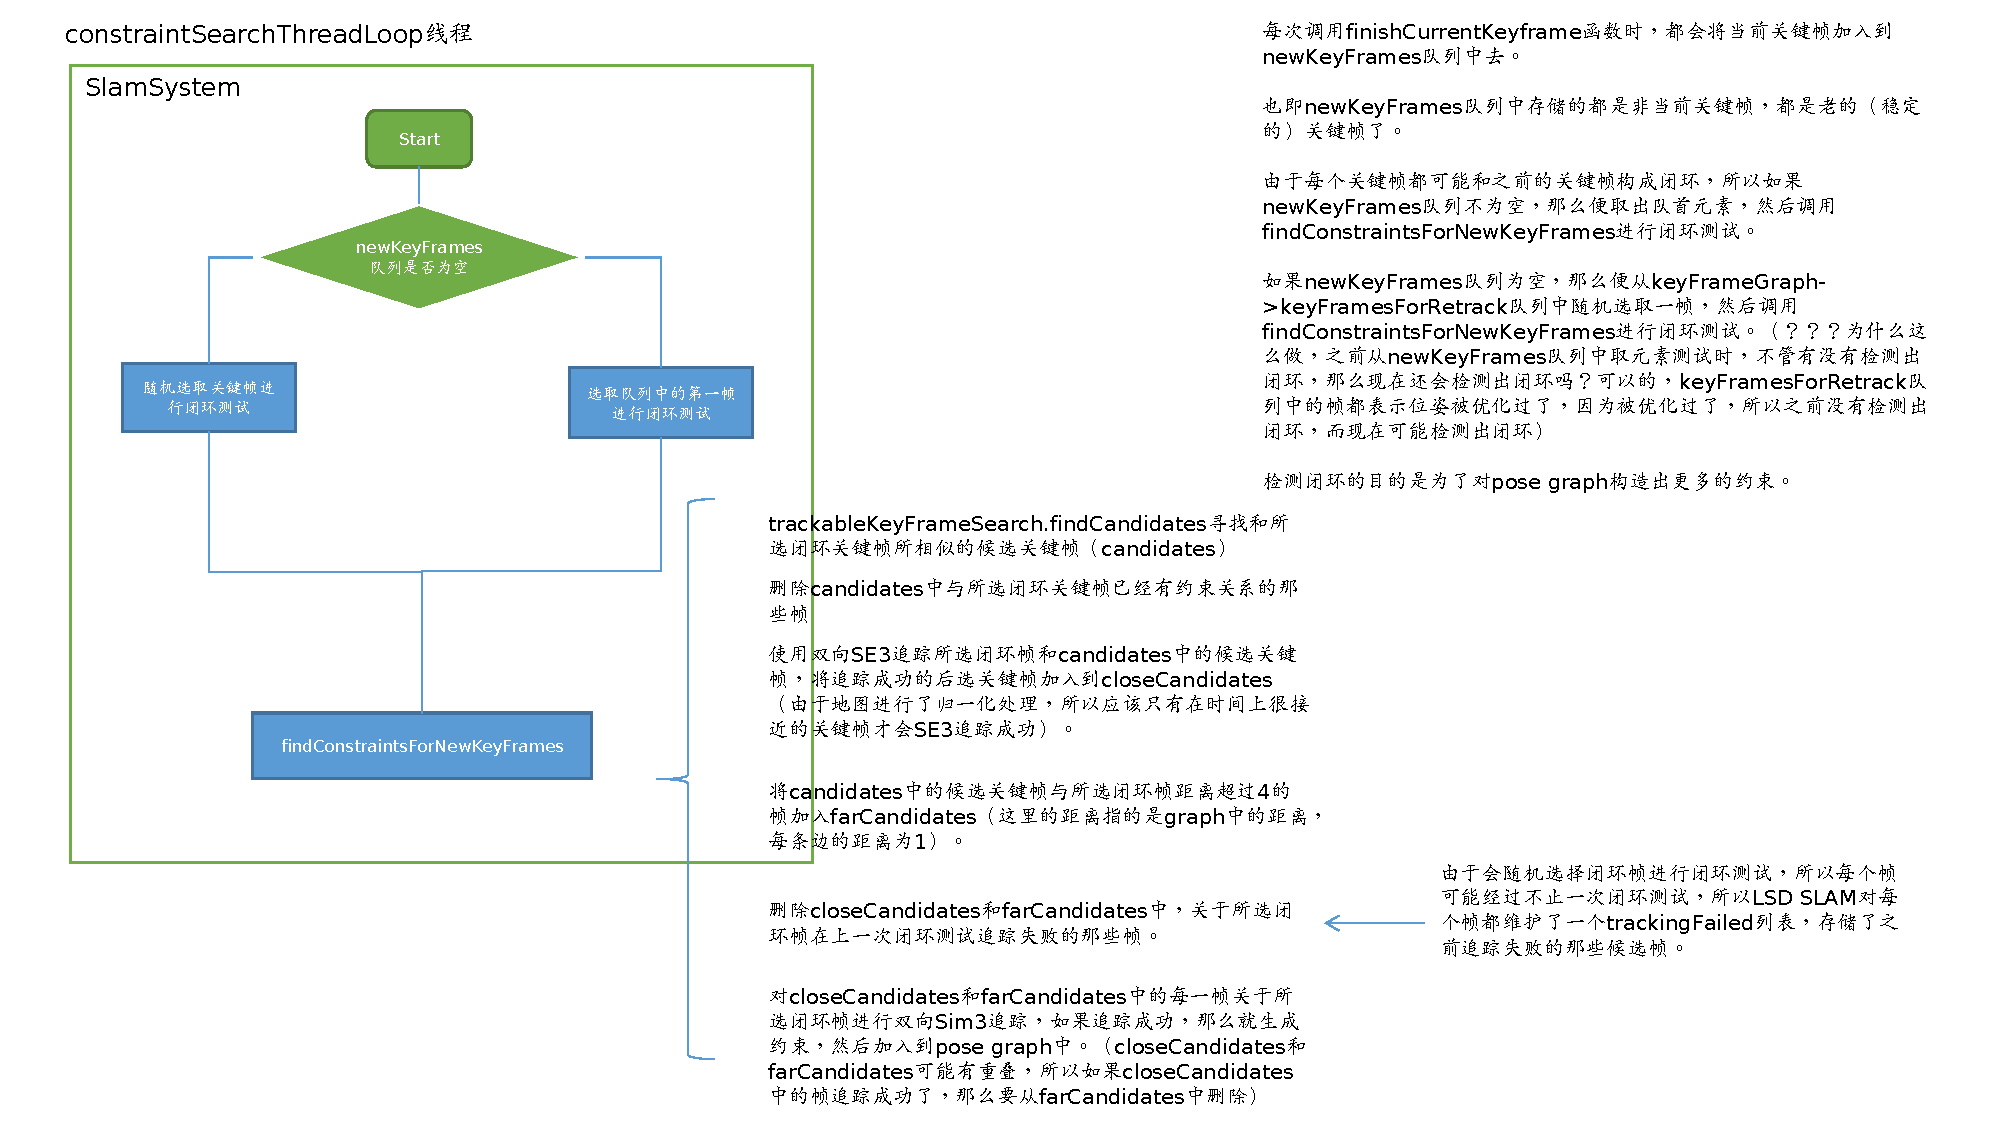
\includegraphics[width=1.0\linewidth]{image/LSD-SLAM/LSD-SLAM-constraint.pdf}  %插入的图,包括JPG,PNG,PDF,EPS等,放在源文件目录下
	\caption{constraintSearchThreadLoop流程图.}  %图片的名称
	\label{fig:constraint_search_thread}   %标签,用作引用
\end{figure}



\section{Optimization}

优化的话,就是对之前构建的pose graph进行优化。
\begin{figure}[h]%%图
	\centering  %插入的图片居中表示
	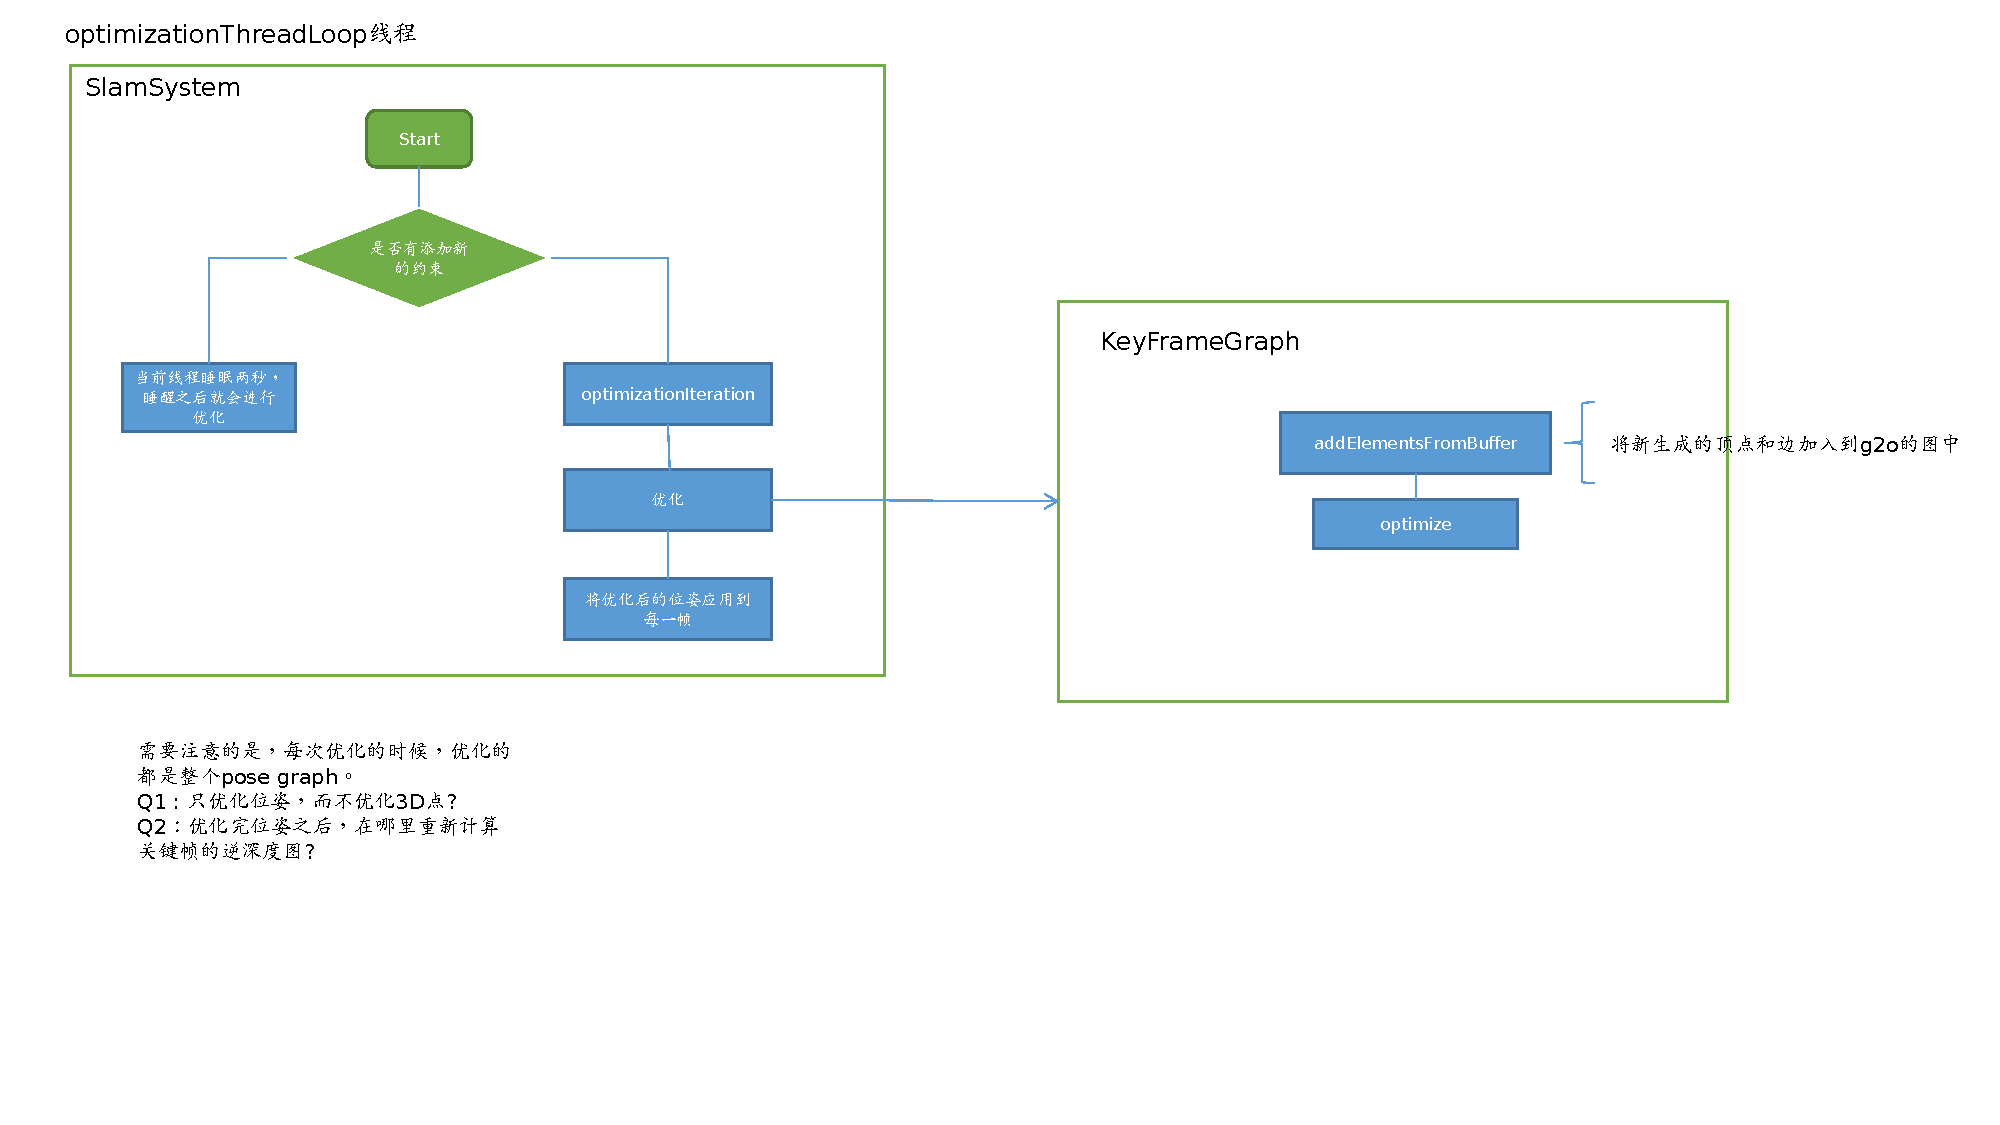
\includegraphics[width=1.0\linewidth]{image/LSD-SLAM/LSD-SLAM-optimization.pdf}  %插入的图,包括JPG,PNG,PDF,EPS等,放在源文件目录下
	\caption{optimizationThread流程图.}  %图片的名称
	\label{fig:optimization_thread}   %标签,用作引用
\end{figure}
\chapter{ORB SLAM}

\section{特征提取--ORBextractor}


\begin{figure}[h]%%图
	\centering  %插入的图片居中表示
	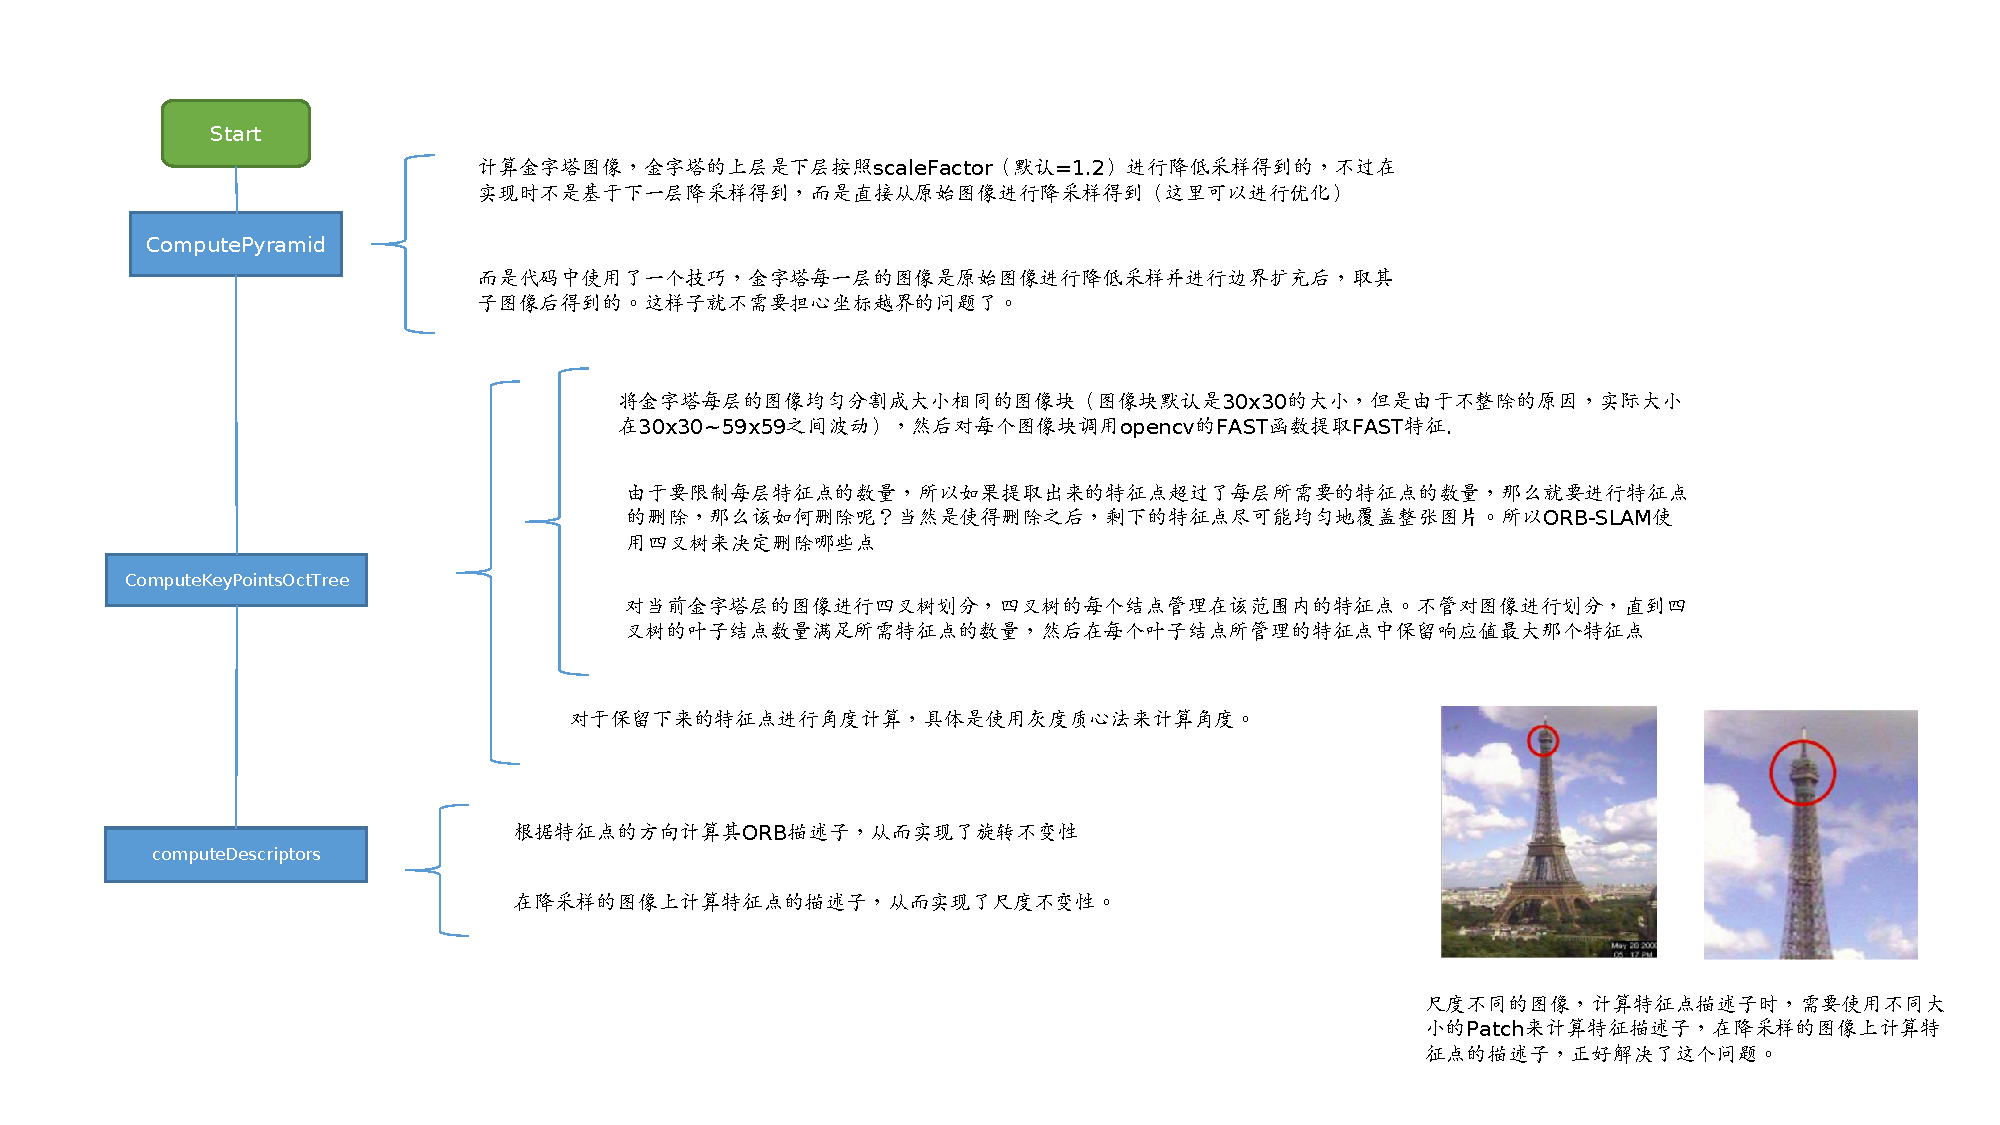
\includegraphics[width=1.0\linewidth]{image/ORB-SLAM/ORBextractor.pdf}  %插入的图,包括JPG,PNG,PDF,EPS等,放在源文件目录下
	\caption{ORB特征提取流程图.}  %图片的名称
	\label{fig:orb_extractor}   %标签,用作引用
\end{figure}


下面是ORB-SLAM构造金字塔的代码:
\begin{lstlisting}[language = C++]
void ORBextractor::ComputePyramid(cv::Mat image)
{
	for (int level = 0; level < nlevels; ++level)
	{
		float scale = mvInvScaleFactor[level];
		// 这是根据尺度进行降采样之后的图像大小
		Size sz(cvRound((float)image.cols*scale), cvRound((float)image.rows*scale));
		// 这是在降采样之后的图像上加上边界之后的大小
		Size wholeSize(sz.width + EDGE_THRESHOLD*2, sz.height + EDGE_THRESHOLD*2);
		Mat temp(wholeSize, image.type()), masktemp;
		// 将temp中的图像部分,非边界部分,赋值到mvImagePyramid
		mvImagePyramid[level] = temp(Rect(EDGE_THRESHOLD, EDGE_THRESHOLD, sz.width, sz.height));
		
		// Compute the resized image
		if( level != 0 )
		{
			resize(mvImagePyramid[level-1], mvImagePyramid[level], sz, 0, 0, INTER_LINEAR);
			
			copyMakeBorder(mvImagePyramid[level], temp, EDGE_THRESHOLD, EDGE_THRESHOLD, EDGE_THRESHOLD, EDGE_THRESHOLD,
			BORDER_REFLECT_101+BORDER_ISOLATED);            
		}
		else
		{
			copyMakeBorder(image, temp, EDGE_THRESHOLD, EDGE_THRESHOLD, EDGE_THRESHOLD, EDGE_THRESHOLD,
			BORDER_REFLECT_101);            
		}
	}
	
}
\end{lstlisting}
ORB-SLAM在构造金字塔时用到了一个技巧,其中\textbf{sz}是降采样之后的图像大小;\textbf{wholeSize}是降采样之后的图像加上边界之后的大小;图像temp的大小是\textbf{wholeSize},接着将图像temp的非边界部分(降采样的图像区域,此时该区域还没有内容)赋值给mvImagePyramid,之后计算ORB特征点时,用到的是mvImagePyramid,哪怕其坐标越界(不要越界太多),那么都是没有问题的。




ORB-SLAM在计算特征点角度时,使用了灰度质心法。需要注意的是,其使用的是圆形patch来计算方向的,所以就必须要知道圆形patch的每一行有多长。ORBextractor在初始化的时候就预计算了圆形patch的每一行有多长(实际上是每一行长度的一半)并存储在umax数组中。



\section{特征匹配--ORBmatcher}

ORBMatcher中的匹配大致分为两种:一种是图像帧知道位姿的匹配;另一种是图像帧不知道位姿的匹配。

\begin{enumerate}
	\item \textbf{已知图像帧位姿的特征点匹配}:因为已知图像帧位姿,所以能够3D点投影到该图像帧上,然后在投影点的周围搜索匹配,从而得到2D-3D点匹配。
	\item \textbf{未知图像帧位状的特征点匹配}:如果不知道图像位姿,那么则使用BoW向量来进行匹配,实际上是通过DBoW2得到的FeatureVector来快速计算特征点之间的匹配。由于正确的特征点匹配一般在Vocabulary Tree上是属于同一个结点的,所以只需要在两张图像帧上,在属于同一个结点的特征点之间进行匹配。
\end{enumerate}

上面的两种匹配策略,都限制了每个特征点所需要测试的特征点数量,从而提高了特征点匹配的效率。




\section{帧间追踪--Tracking线程}

Tracking线程的流程如图\ref{fig:orb_tracking}所示。

\begin{figure}[h]%%图
	\centering  %插入的图片居中表示
	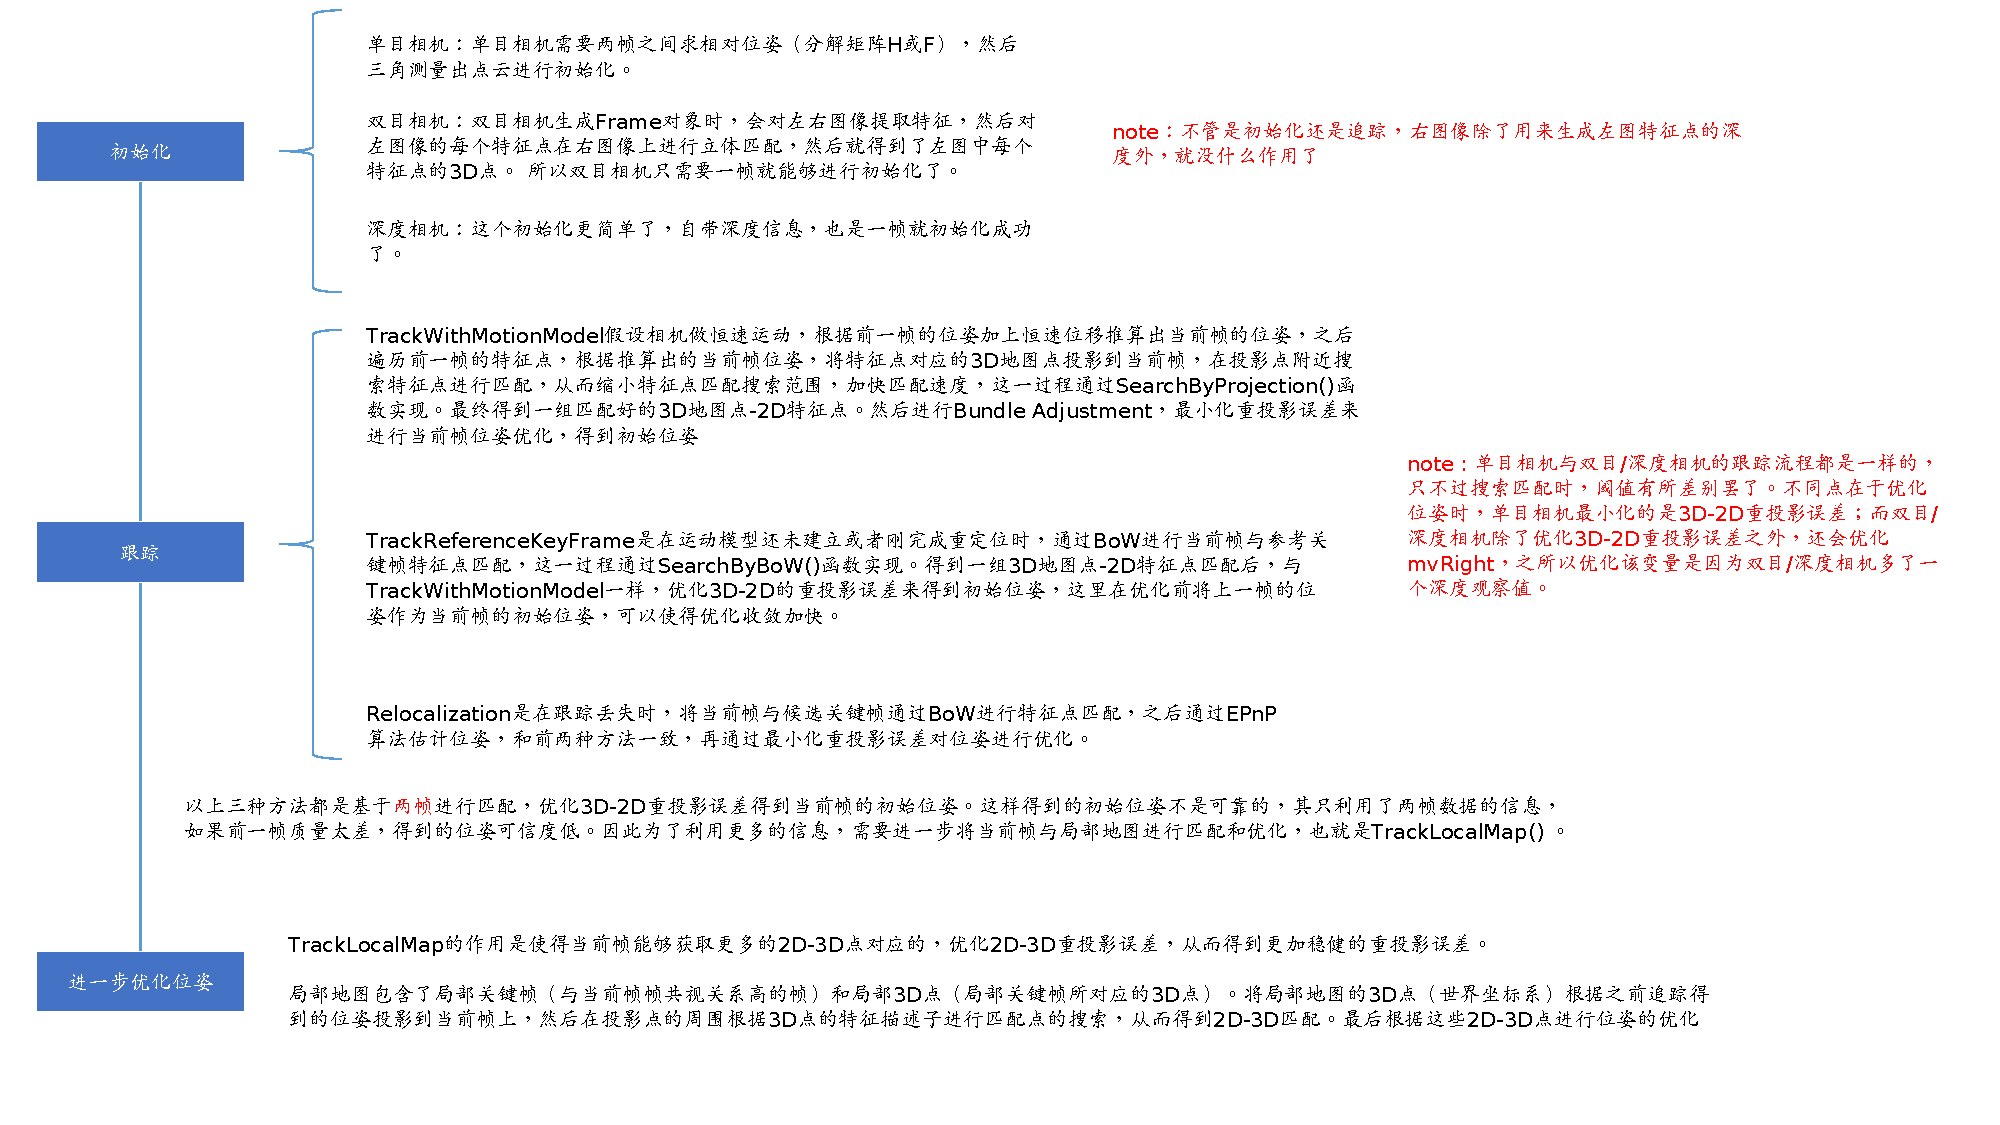
\includegraphics[width=1.0\linewidth]{image/ORB-SLAM/Tracking.pdf}  %插入的图,包括JPG,PNG,PDF,EPS等,放在源文件目录下
	\caption{帧间跟踪流程图.}  %图片的名称
	\label{fig:orb_tracking}   %标签,用作引用
\end{figure}





\section{局部建图--LocalMapping线程}

ORB-SLAM2中的LocalMapping线程是用来对\textbf{关键帧}进行建图的,也即尽可能恢复关键帧中2D特征点所对应的3D点的坐标,其流程如图\ref{fig:local_mapping}所示。

Tracking线程会将创建好的关键帧插入到LocalMapping线程的队列中,而LocalMapping线程要做的就是不断取出队列中的关键帧,对其进行建图。

\begin{enumerate}
	\item LocalMapping取出队首第一帧之后,先是处理该关键帧已有的2D-3D对应关系(追踪该关键帧时,所得到的2D-3D点对应关系),其实就是将2D点添加为3D点的观测;
	\item 然后就是删除一些不稳定、或是错误的3D点,LocalMapping线程会维护一个mlpRecentAddedMapPoings列表,该列表存储了一些最近新三角测量得到的3D点,在经过一段时间后,如果某些3D点的observation数量太少的话,那么就说明该3D点不稳定、或者是错误的,则会被删除;
	\item 接着就是对该关键帧上那些没有3D点对应的2D点进行三角测量了,对于没有3D点对应的2D点在该关键帧的相邻关键帧上寻找匹配点(利用BoW寻找匹配),对于找到的匹配点进行极线验证,对于通过极线验证的2D-2D匹配点才会进行三角测量,对于单目相机,肯定是进行三角测量,而对于双目/深度相机,则有可能使用其自带的深度信息而不进行三角测量。得到3D点后,还需要进行一系列的检测才会决定创不创建该3D点为MapPoint,具体的条件为深度在两帧图像上为正,在两帧图像上的重投影误差不能太大等。
	\item 在创建完新的3D点之后,如果当前线程空闲(也即关键帧队列为空),那么就进行3D点的融合处理。因为ORB-SLAM2进行的是\textbf{二视图三角测量},而一个3D点的观测(2D点)可能会出现在很多张图像上,这样子就会导致三角测量出多个3D点,3D点融合要做的就是让这些2D点(观测)变成同一个3D点的observation。\begin{enumerate}[(1)]
		\item 将当前关键帧的3D点投影到其相邻关键帧上,然后在一定的半径内找到2D匹配点(找到特征描述子距离最小的匹配点,并且该距离要小于阈值,因为距离最小并不代表就是匹配点,因此还要判断距离阈值)进行融合。融合的方法是:(a)如果该2D点没有3D点对应,那么就让该2D点称为当前关键帧3D点的observation;(b)如有该2D点存在3D点对应,那么现在就有了两个3D点了,根据哪个3D点的observation多(稳定),那么就以哪个3D点为准,并且融合两个3D点的observation。
		\item 将相邻关键帧的3D点投影到当前关键帧,然后找到匹配点,进行融合。
		\end{enumerate}
	\item 最后,删除冗余的关键帧。如果该关键帧90\%的3D点都能在其某个相邻关键帧上看到,那么就认为该关键帧是冗余的,可以删除。

\end{enumerate}



\begin{figure}[h]%%图
	\centering  %插入的图片居中表示
	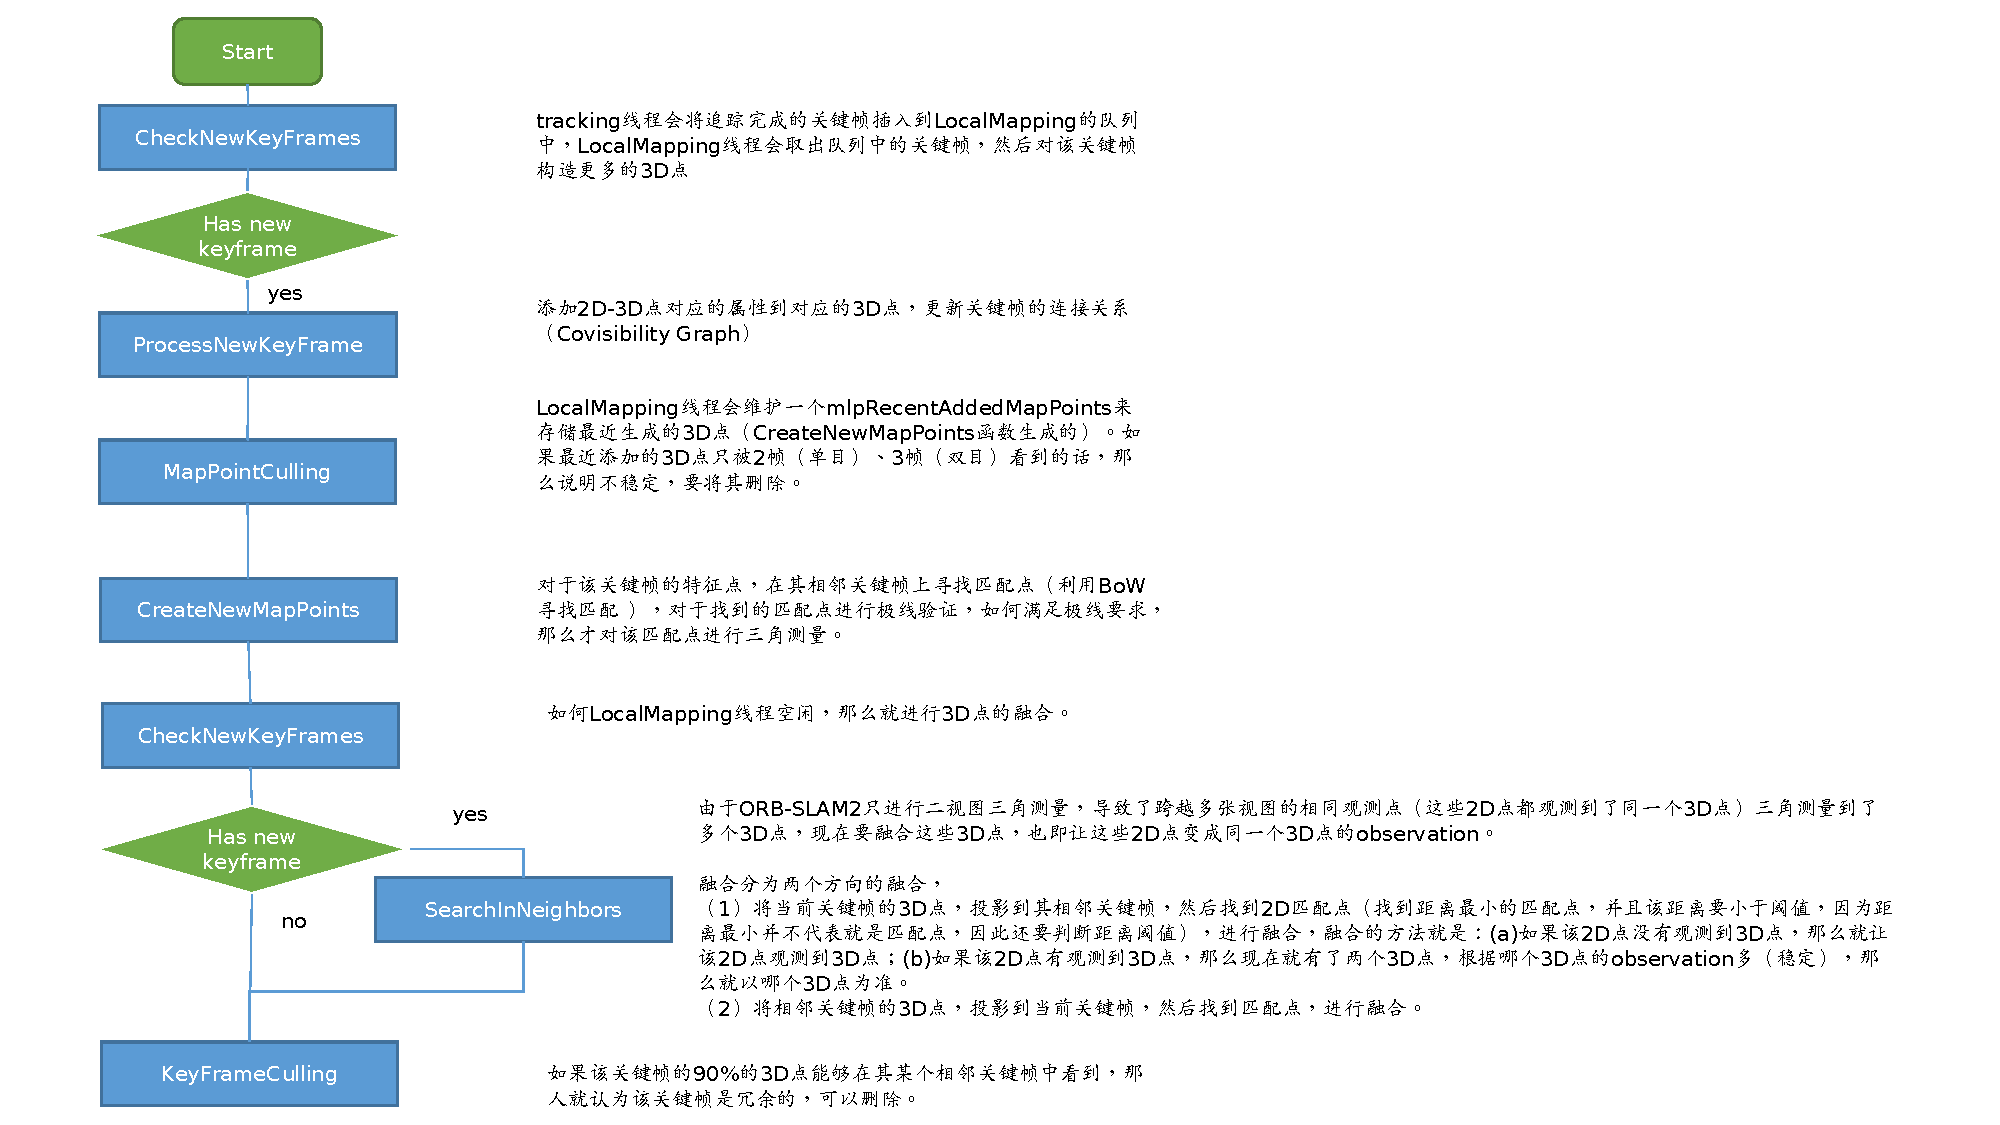
\includegraphics[width=1.0\linewidth]{image/ORB-SLAM/LocalMapping.pdf}  %插入的图,包括JPG,PNG,PDF,EPS等,放在源文件目录下
	\caption{ORB-SLAM2局部建图流程图.}  %图片的名称
	\label{fig:local_mapping}   %标签,用作引用
\end{figure}





\section{闭环修复--LoopClosing线程}



下面只讨论检测到闭环后如何修复闭环,至于如何检测闭环,就不细说了。

\begin{figure}[h]%%图
	\centering  %插入的图片居中表示
	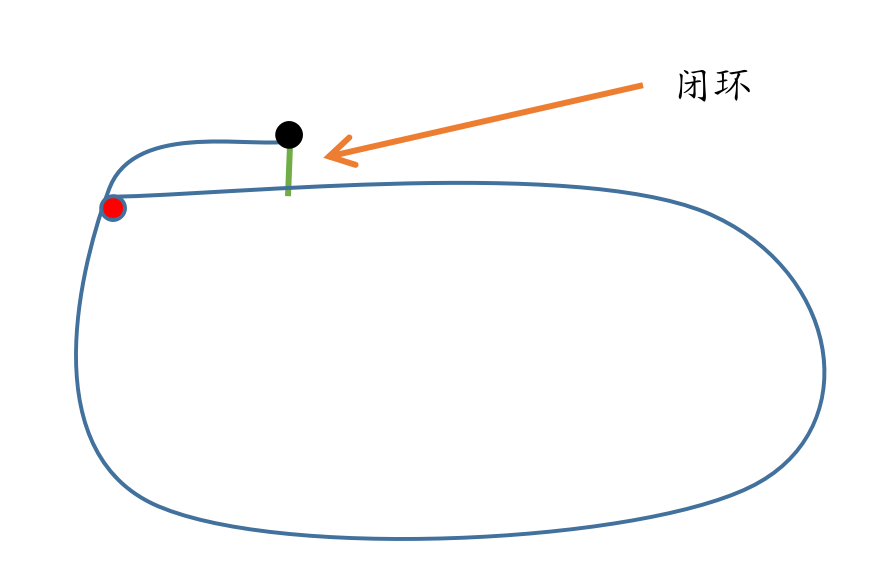
\includegraphics[width=0.4\linewidth]{image/ORB-SLAM/DetectedLoop.png}  %插入的图,包括JPG,PNG,PDF,EPS等,放在源文件目录下
	\caption{检测闭环成功.红点代表起始位置,黑点代表终止位置,绿线代表两张图像相似.}  %图片的名称
	\label{fig:detected_loop}   %标签,用作引用
\end{figure}



图\ref{fig:detected_loop}是闭环检测成功之后的示意图。检测到闭环之后,我们就可以利用闭环关键帧的位姿(累积误差小)来计算得到当前关键帧的位姿,从而减少当前关键帧位姿的累积误差。\textbf{首先},我们要做的就是计算当前关键帧和闭环关键帧之间的Sim3变换(通过对齐两帧之间的3D点得到)。\textbf{然后},由于当前关键帧的点云和闭环关键帧的点云之间相差一个Sim3变换,那么当前关键帧的位姿和闭环关键帧之间的位姿也是相差该Sim3变换(\textbf{note}:想一想3D-3D点对应是如何求位姿的),根据这个原理就能对当前关键帧的位姿进行修复,相当于使用闭环关键帧的位姿计算得到当前关键帧的位姿,从而减少了累积误差。

具体对当前关键帧的位姿进行修复的公式如下:

\begin{equation}
	mg2oScw = gScm * gSmw
\end{equation}
其中,$mg2oScw$表示当前关键帧修复后的位姿,$gScm$表示闭环关键帧到当前关键帧的相对变换Sim3,$gSmw$表示闭环关键帧的绝对位姿(世界坐标系到闭环帧坐标系的变换。该公式就是利用了闭环关键帧的位姿(误差小)计算得到了当前关键帧的位姿,从而减少了当前关键帧位姿的累积误差。


\begin{figure}[h]%%图
	\centering  %插入的图片居中表示
	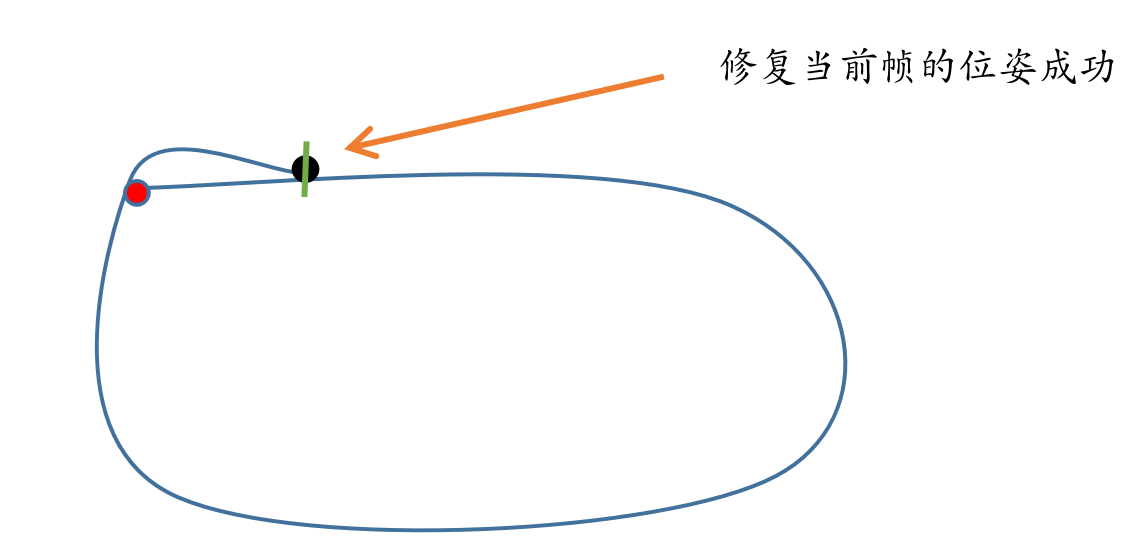
\includegraphics[width=0.5\linewidth]{image/ORB-SLAM/LoopFix1.png}  %插入的图,包括JPG,PNG,PDF,EPS等,放在源文件目录下
	\caption{修复当前关键帧位姿成功.}  %图片的名称
	\label{fig:loop_fix1}   %标签,用作引用
\end{figure}


图\ref{fig:loop_fix1}是当前关键帧对位姿进行修复后的示意图。可见,单单修复当前关键帧的位姿是不行的,还需要修复整个环上其它关键帧的位姿。\textbf{首先},从修复当前关键帧的相邻关键帧(共视关键帧)开始,因为当前关键帧的相邻关键帧是能够看到相同3D点的关键帧,那么当前关键帧通过和闭环关键帧对齐3D点得到的Sim3也是能够用到相邻关键帧上的,那么就也对相邻关键帧的位姿进行了修复。



对当前关键帧的相邻关键帧的位姿进行修复的公式如下:


\begin{equation}
\begin{split}
g2oCorrectedSiw& = g2oSic * mg2oScw \\
&=  g2oSic * gScm * gSmw
\end{split}
\end{equation}

其中,$g2oSic$表示当前关键帧到其第i个相邻关键帧的相对位姿,$mg2oScw$表示当前关键帧修复后的位姿。




\begin{figure}[h]%%图
	\centering  %插入的图片居中表示
	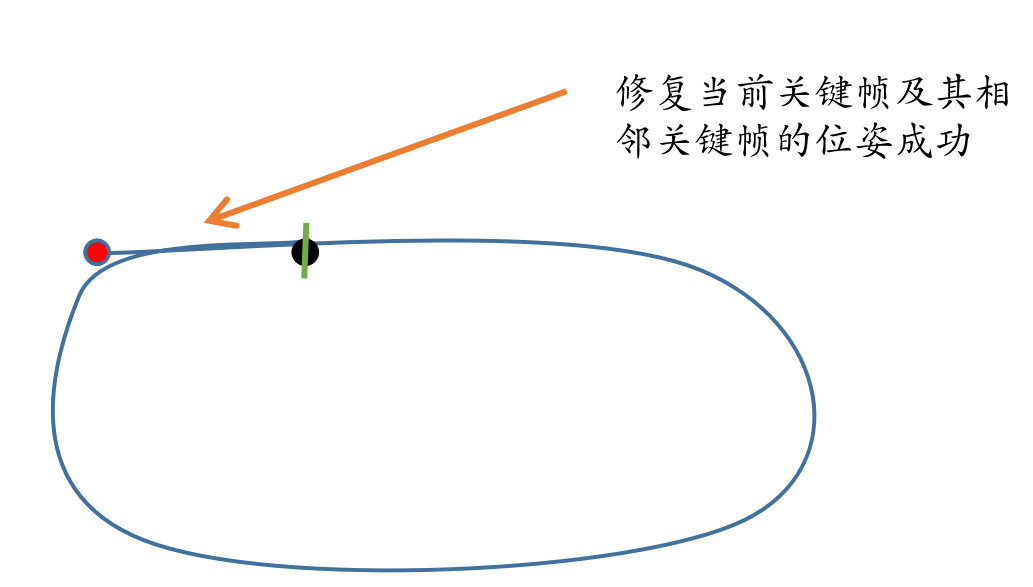
\includegraphics[width=0.5\linewidth]{image/ORB-SLAM/LoopFix2.png}  %插入的图,包括JPG,PNG,PDF,EPS等,放在源文件目录下
	\caption{修复当前关键帧及其相邻关键帧位姿成功.}  %图片的名称
	\label{fig:loop_fix2}   %标签,用作引用
\end{figure}


图\ref{fig:loop_fix2}是修复当前关键帧及其相邻关键帧位姿成功之后的示意图。到此,已经修复了当前关键帧及其相邻关键帧的位姿。但是,如果仅仅修复这些关键帧的位姿的话,没有修复剩余的帧的话,那么就会造成不一致(哪里不一致?),所以就要对剩余的位姿进行修复。而这些关键帧位姿的修复就交给了pose graph optimization。当然了,只要能够最小化整体的误差,pose graph optimization时也会对当前关键帧及其相邻关键帧的位姿进行调整。

那么就下来就是要构造pose grpah了,那么ORB-SLAM2是如何构造pose graph的呢?ORB-SLAM2对所有的关键帧构造一个pose graph,然后对其进行优化。

\textbf{构造顶点},pose graph的顶点(待优化变量)为关键帧的绝对位姿,对于当前关键帧及其相邻关键帧,其绝对位姿就是修复过后的位姿;而对于其它关键帧,其位姿就是原来的位姿;并且优化时,闭环关键帧的位姿被设置为不变,只作为约束条件。

\textbf{构造边},pose graph的边(约束条件)为关键帧之间的相对位姿,那么ORB-SLAM2往pose graph中插入了哪些边呢?

\begin{itemize}
	\item 当前关键帧及其相邻关键帧之间的相对位姿,如图\ref{fig:more_loop_constarint}所示;
	\item 每个关键帧与父亲之间的相对位姿;
	\item 每个关键帧与其回环边之间的相对位姿(不是每个关键帧都有回环边的),每次pose graph optimization之后,都会在当前关键帧和闭环关键帧之间添加一条双向的边。每次进行pose graph optimization时,都会将之前pose graph optimization时生成的回环边加入进来;
	\item 每个关键帧及其相邻关键帧之间的相对位姿。
\end{itemize}

\begin{figure}[h]%%图
	\centering  %插入的图片居中表示
	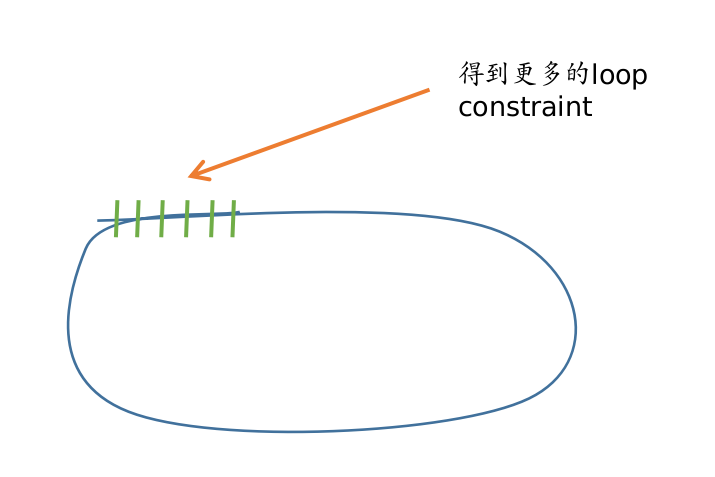
\includegraphics[width=0.5\linewidth]{image/ORB-SLAM/MoreLoopConstraint.png}  %插入的图,包括JPG,PNG,PDF,EPS等,放在源文件目录下
	\caption{当前关键帧及其相邻关键帧的loop constraint.}  %图片的名称
	\label{fig:more_loop_constarint}   %标签,用作引用
\end{figure}

如何ORB-SLAM2是如何计算这些相对位姿(约束条件)的呢?如图\ref{fig:loop_constraint}所示。为什么有时使用\textbf{修复后}的位姿计算相对位姿,有时使用\textbf{修复前}的位姿计算相对位姿呢?

对于第一种情况,使用修复后的位姿计算相对位姿很好理解,因为闭环关键帧及其周围帧的位姿被认为是正确的,那么通过它们修复的当前关键帧及其相邻关键帧的位姿也是正确的,那么它们之间的相对位姿,自然是使用修复过后的位姿进行计算;

至于后面的三种情况,试想一下,如果边的一边是修复后的位姿(当前关键帧或其相邻关键帧的位姿),一边是没有修复的位姿态(除了当前关键帧及其相邻关键帧之外的帧的位姿),那么计算得到的相对位姿肯定是错的,所以要使用\textbf{未修复}之前的位姿来计算相对位姿,通过该约束,从而对边的另一边未修复的位姿进行优化。

\begin{figure}[h]%%图
	\centering  %插入的图片居中表示
	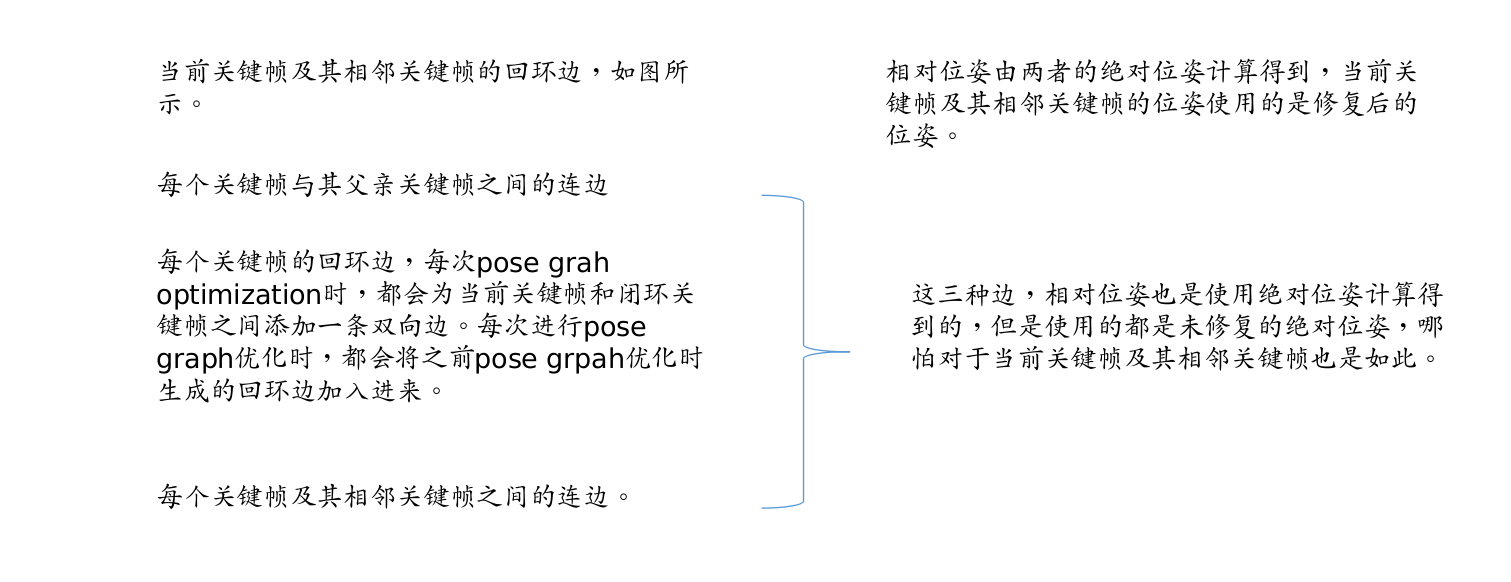
\includegraphics[width=1.0\linewidth]{image/ORB-SLAM/LoopConstraint.png}  %插入的图,包括JPG,PNG,PDF,EPS等,放在源文件目录下
	\caption{ORB-SLAM2如何计算相对位姿.}  %图片的名称
	\label{fig:loop_constraint}   %标签,用作引用
\end{figure}


\begin{note}
	对于pose graph optimization,其成立的基础是相对位姿是准的,但是ORB-SLAM2中的相对位姿是通过绝对位姿计算得到的,既然绝对位姿都是不准的,那么通过其计算得到的相对位姿能是准的吗???
\end{note}


\textbf{姑且认为相对位姿是准的吧},pose graph以相对位姿作用约束,通过优化绝对位姿,减少了误差,并且误差分布到了整个pose graph的顶点上,所以通过pose graph优化后,SLAM的效果能够好很多。但是pose graph优化的前提是检测到闭环,如果SLAM一直前进,不会回到原来走过的地方,那么pose graph也没什么办法。



下面完整地介绍下闭环处理的流程:
\begin{enumerate}
	\item Loop detection
	\item Loop closing
	\item Loop correction
\end{enumerate}

Loop detection就是判断当前走过的地方是不是之前走过的,如果之前就走过了,那么就产生了闭环;Loop closing则是通过闭环关键帧计算得到当前关键帧的位姿,从而减少当前关键帧的累积误差;而Loop correction则是使用pose graph optimization,将闭环得到的信息传播给其它的关键帧,从而减少了其它关键帧的累积误差。



在进行pose graph optimization之后,就要对3D点的位置进行修正。首先,对于每个3D点得到其reference keyframe,也就是哪个关键帧创建了该3D点;然后使用该帧旧的位姿将该3D点转换到该关键帧的坐标系下,然后再使用优化过后的位姿将3D点反投影回到世界坐标系,那么就得到了\textbf{修正}过后的3D点坐标。

在使用pose graph对位姿进行优化,以及使用优化过后的位姿对3D点的坐标进行修正后,LoopClosing线程最后会调用GlobalBundleAdjustment对位姿和3D点进行联合优化。



\section{总结}
ORB-SLAM2中重要的模块差不多就是\textbf{特征点提取}、\textbf{初始化}、\textbf{跟踪}(求下一帧图像的位姿)、\textbf{建图}、\textbf{回环检测}、\textbf{优化}。

\textbf{特征点提取}。对每帧图像提取ORB特征点,并在OpenCV的ORB特征提取的基础上进行改进,使其提取出来的特征在图像上的分布更加均匀。

\textbf{初始化}。单目相机和双目/深度相机的初始化是不同的。双目/深度由于自带深度,所以只需要一帧(对于双目相机来说,这里说的一帧表示同一时刻拍摄的左右帧)就能够完成初始化。而对于单目相机而言,由于缺少了深度相机,所以需要两帧图像才能够完成初始化,单目相机初始化时,需要通过分解\textbf{单应矩阵}H或\textbf{本质矩阵}E来得到位姿,并且通过该位姿对2D-2D特征点对应进行三角测量得到3D点,从而完成单目相机的初始化。

\textbf{跟踪}。跟踪就是不断求下一帧图像位姿的过程。对于SFM来说,一般来说都是通过与一帧图像进行匹配得到2D-2D点对应,并根据传递性,从而得到2D-3D点对应,接着使用PnP来求解位姿。而对于ORB-SLAM2来说,也是通过传递性找到2D-3D点对应,但是ORB-SLAM2并没有使用PnP来求解位姿,而是通过最小化误差来得到下一帧图像的位姿的。对于单目相机,最小化的是重投影误差,对于双目/深度相机,最小化的是立体特征$(u_L, v_L, u_R)$的误差?

\textbf{关键帧选取}。这个判断的条件那是相当复杂,需要看代码才能懂ORB-SLAM2是如何选取关键帧的。不过简单地说的话,就是相距当前关键帧相机移动了一定的距离才需要添加,不过ORB-SLAM2判断的不是距离,而是通过各种2D、3D点的数量来判断相机移动远了,也即是否需要添加关键帧。

\textbf{建图}。跟踪部分对每一帧图像都进行跟踪,而建图则只对那些被选为关键帧的图像帧进行建图。跟踪部分是最小化2D-3D点对应的重投影误差来得到下一帧的位姿的,但是此时下一帧中某些2D点是没有3D点对应的,我们要恢复这部分2D点所对应的3D点,也就是叫做建图了。下一帧关键帧根据Covisibility Graph找到与其相邻的图像帧,并寻找2D-2D点匹配,然后通过三角测量得到新的3D点。

\textbf{回环检测}。回环检测就是通过检测到SLAM过程中是否来到之前已经走过的地方,通过之前帧的位姿来计算当前帧的位姿,从而减少当前帧位姿的累积误差,并且也重新计算当前帧相邻帧的位姿,也减少了这些相邻帧的累积误差。之后,将这个信息传播到整个pose graph上,通过优化pose graph,将累积误差减少的同时,将误差分布到整个pose graph时,从而使得整个SLAM的结果更好。当然,pose graph优化的弊端是必须经过相同的地方,如果SLAM过程中一直往前走,那么pose graph的效果并不会很好。

\textbf{优化}。优化部分包含LocalBundleAdjustment、OptimizeEssentialGraph以及GlobalBundleAdjustment。LocalBundleAdjustment会在局部建图之后,LocalMapping线程空闲时才会调用(没有关键帧需要建图)。OptimizeEssentialGraph就是用在了回环检测上。而GlobalBundleAdjustment之后再纠正闭环之后才会调用。



\section{参考文献}

【AR实验室】mulberryAR:并行提取ORB特征
https://www.cnblogs.com/polobymulberry/p/6270399.html


[ORB-SLAM2] ORB特征提取策略对ORB-SLAM2性能的影响
https://zhuanlan.zhihu.com/p/57235987


[ORB-SLAM2]卡方分布(Chi-squared)外点(outlier)剔除
https://zhuanlan.zhihu.com/p/58556978

orbslam作者的ppt
https://blog.csdn.net/u012700322/article/details/51965152

ORB\_SLAM2中的Sim3优化
https://zhehangt.github.io/2018/11/01/SLAM/ORBSLAM/ORBSLAM2LoopClosingRefine/


ORB-SLAM2从理论到代码实现(五):ORBmatcher.cc程序详解
https://blog.csdn.net/qq\_20123207/article/details/82502207

Loop Closing 3d Point Clouds
https://stackoverflow.com/questions/37279020/loop-closing-3d-point-clouds


ORB-SLAM(十)LoopClosing Sim3求解
https://www.cnblogs.com/shang-slam/p/6480863.html


Scale Drift Issue \#71
https://github.com/raulmur/ORB\_SLAM2/issues/71




\chapter{DSO SLAM}

\chapter{Vins SLAM}


\chapter{漫谈SLAM}

摘录自 https://www.cnblogs.com/qcloud1001/p/7978238.html

https://cloud.tencent.com/developer/article/1005893

\section{漫谈 SLAM 技术(上)}
随着最近几年机器人、无人机、无人驾驶、VR/AR的火爆,SLAM技术也为大家熟知,被认为是这些领域的关键技术之一。本文对SLAM技术及其发展进行简要介绍,分析视觉SLAM系统的关键问题以及在实际应用中的难点,并对SLAM的未来进行展望。

\subsection{SLAM技术}

SLAM(Simultaneous Localization and Mapping),同步定位与地图构建,最早在机器人领域提出,它指的是:机器人从未知环境的未知地点出发,在运动过程中通过重复观测到的环境特征定位自身位置和姿态,再根据自身位置构建周围环境的增量式地图,从而达到同时定位和地图构建的目的。由于SLAM的重要学术价值和应用价值,一直以来都被认为是实现全自主移动机器人的关键技术。

如下图,通俗的来讲,SLAM回答两个问题:“我在哪儿?”“我周围是什么?”,就如同人到了一个陌生环境中一样,SLAM试图要解决的就是恢复出观察者自身和周围环境的相对空间关系,“我在哪儿”对应的就是定位问题,而“我周围是什么”对应的就是建图问题,给出周围环境的一个描述。回答了这两个问题,其实就完成了对自身和周边环境的空间认知。有了这个基础,就可以进行路径规划去达要去的目的地,在此过程中还需要及时的检测躲避遇到的障碍物,保证运行安全。

\begin{figure}[h]%%图
	\centering  %插入的图片居中表示
	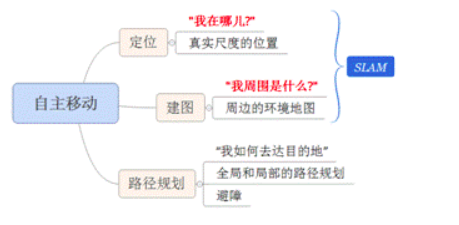
\includegraphics[width=0.7\linewidth]{image/Talk/1.png}  %插入的图,包括JPG,PNG,PDF,EPS等,放在源文件目录下
	\caption{SLAM概念}  %图片的名称
\end{figure}

\subsection{SLAM发展简介}
自从上世纪80年代SLAM概念的提出到现在,SLAM技术已经走过了30多年的历史。SLAM系统使用的传感器在不断拓展,从早期的声呐,到后来的2D/3D激光雷达,再到单目、双目、RGBD、ToF等各种相机,以及与惯性测量单元IMU等传感器的融合;SLAM的算法也从开始的基于滤波器的方法(EKF、PF等)向基于优化的方法转变,技术框架也从开始的单一线程向多线程演进。下面介绍这些过程中一些代表性的SLAM技术。

(1)激光雷达SLAM发展

基于激光雷达的SLAM(Lidar SLAM)采用2D或3D激光雷达(也叫单线或多线激光雷达),如下图所示。在室内机器人(如扫地机器人)上,一般使用2D激光雷达,在无人驾驶领域,一般使用3D激光雷达。


\begin{figure}[h]%%图
	\centering  %插入的图片居中表示
	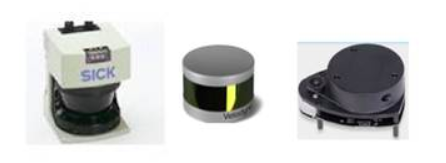
\includegraphics[width=0.7\linewidth]{image/Talk/2.png}  %插入的图,包括JPG,PNG,PDF,EPS等,放在源文件目录下

\end{figure}


激光雷达的优点是测量精确,能够比较精准的提供角度和距离信息,可以达到<1°的角度精度以及cm级别的测距精度,扫描范围广(通常能够覆盖平面内270°以上的范围),而且基于扫描振镜式的固态激光雷达(如Sick、Hokuyo等)可以达到较高的数据刷新率(20Hz以上),基本满足了实时操作的需要;缺点是价格比较昂贵(目前市面上比较便宜的机械旋转式单线激光雷达也得几千元),安装部署对结构有要求(要求扫描平面无遮挡)。

激光雷达SLAM建立的地图常常使用占据栅格地图(Ocupanccy Grid)表示,每个栅格以概率的形式表示被占据的概率,存储非常紧凑,特别适合于进行路径规划。

\begin{figure}[h]%%图
	\centering  %插入的图片居中表示
	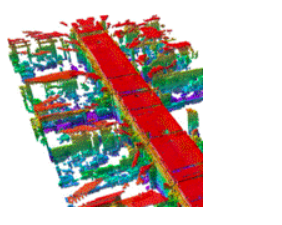
\includegraphics[width=0.7\linewidth]{image/Talk/3.png}  %插入的图,包括JPG,PNG,PDF,EPS等,放在源文件目录下
	\caption{激光雷达.}  %图片的名称
\end{figure}

现任Udacity创始人CEO、前Google副总裁、谷歌无人车领导者Sebastian Thrun大神(下图)在他2005年的经典著作《Probabilistic Robotics》一书中详细阐述了利用2D激光雷达基于概率方法进行地图构建和定位的理论基础,并阐述了基于RBPF粒子滤波器的FastSLAM方法,成为后来2D激光雷达建图的标准方法之一GMapping[1][2]的基础,该算法也被集成到机器人操作系统(Robot Operation System,ROS)中。
\begin{figure}[h]%%图
	\centering  %插入的图片居中表示
	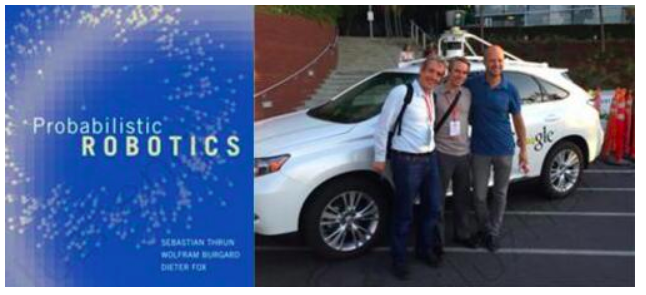
\includegraphics[width=0.7\linewidth]{image/Talk/4.png}  %插入的图,包括JPG,PNG,PDF,EPS等,放在源文件目录下

\end{figure}


2013年,文献[3]对ROS中的几种2D SLAM的算法HectorSLAM,KartoSLAM,CoreSLAM,LagoSLAM和GMapping做了比较评估,读者可前往细看。

2016年,Google开源其激光雷达SLAM算法库Cartographer[4],它改进了GMapping计算复杂,没有有效处理闭环的缺点,采用SubMap和Scan Match的思想构建地图,能够有效处理闭环,达到了较好的效果。

(2)视觉SLAM发展

相比于激光雷达,作为视觉SLAM传感器的相机更加便宜、轻便,而且随处可得(如人人都用的手机上都配有摄像头),另外图像能提供更加丰富的信息,特征区分度更高,缺点是图像信息的实时处理需要很高的计算能力。幸运的是随着计算硬件的能力提升,在小型PC和嵌入式设备,乃至移动设备上运行实时的视觉SLAM已经成为了可能。

视觉SLAM使用的传感器目前主要有单目相机、双目相机、RGBD相机三种,其中RGBD相机的深度信息有通过结构光原理计算的(如Kinect1代),也有通过投射红外pattern并利用双目红外相机来计算的(如Intel RealSense R200),也有通过TOF相机实现的(如Kinect2代),对用户来讲,这些类型的RGBD都可以输出RGB图像和Depth图像。

\begin{figure}[h]%%图
	\centering  %插入的图片居中表示
	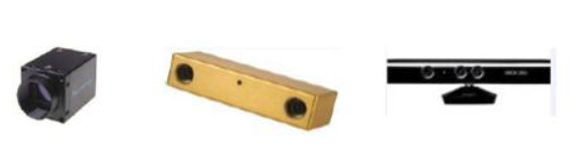
\includegraphics[width=0.7\linewidth]{image/Talk/5.png}  %插入的图,包括JPG,PNG,PDF,EPS等,放在源文件目录下

\end{figure}


现代流行的视觉SLAM系统大概可以分为前端和后端,如下图所示。前端完成数据关联,相当于VO(视觉里程计),研究帧与帧之间变换关系,主要完成实时的位姿跟踪,对输入的图像进行处理,计算姿态变化,同时也检测并处理闭环,当有IMU信息时,也可以参与融合计算(视觉惯性里程计VIO的做法);后端主要对前端的输出结果进行优化,利用滤波理论(EKF、PF等)或者优化理论进行树或图的优化,得到最优的位姿估计和地图。

\begin{figure}[h]%%图
	\centering  %插入的图片居中表示
	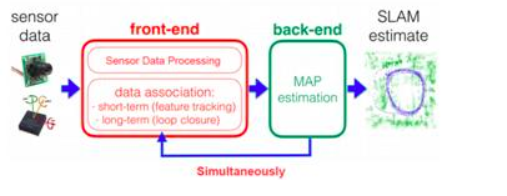
\includegraphics[width=0.7\linewidth]{image/Talk/6.png}  %插入的图,包括JPG,PNG,PDF,EPS等,放在源文件目录下

\end{figure}

采用滤波器的SLAM,如下图(a),估计n时刻的相机位姿Tn需要使用地图中所有路标的信息,而且每帧都需要更新这些路标的状态,随着新的路标的不断加入,状态矩阵的规模增长迅速,导致计算和求解耗时越来越严重,因此不适宜长时间大场景的操作;而采用优化算法的SLAM,如下图(b),通常结合关键帧使用,估计n时刻的相机位姿Tn可以使用整个地图的一个子集,不需要在每幅图像都更新地图数据,因此现代比较成功的实时SLAM系统大都采取优化的方法。
\begin{figure}[h]%%图
	\centering  %插入的图片居中表示
	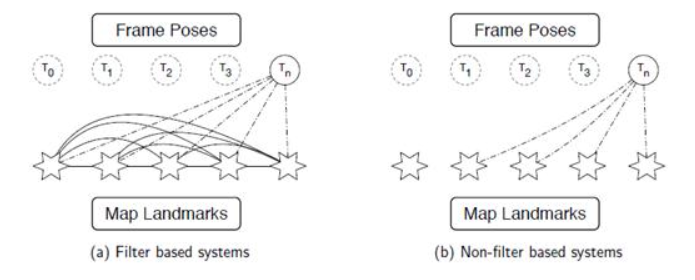
\includegraphics[width=0.7\linewidth]{image/Talk/7.png}  %插入的图,包括JPG,PNG,PDF,EPS等,放在源文件目录下

\end{figure}






下面介绍视觉SLAM发展历程中几个比较有代表性的SLAM系统进行介绍:

MonoSLAM[5]是2007年由Davison 等开发的第一个成功基于单目摄像头的纯视觉SLAM 系统。MonoSLAM使用了扩展卡尔曼滤波,它的状态由相机运动参数和所有三维点位置构成, 每一时刻的相机方位均带有一个概率偏差,每个三维点位置也带有一个概率偏差, 可以用一个三维椭球表示, 椭球中心为估计值, 椭球体积表明不确定程度(如下图所示),在此概率模型下, 场景点投影至图像的形状为一个投影概率椭圆。MonoSLAM 为每帧图像中抽取Shi-Tomasi角点[6], 在投影椭圆中主动搜索(active search)[7]特征点匹配。由于将三维点位置加入估计的状态变量中,则每一时刻的计算复杂度为O(n3) , 因此只能处理几百个点的小场景。
\begin{figure}[H]%%图
	\centering  %插入的图片居中表示
	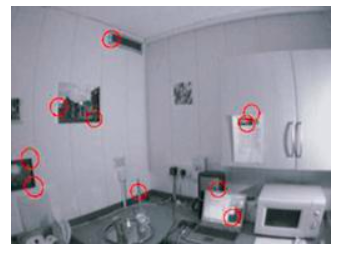
\includegraphics[width=0.7\linewidth]{image/Talk/8.png}  %插入的图,包括JPG,PNG,PDF,EPS等,放在源文件目录下

\end{figure}



同年,Davison在Oxford的师父Murray和Klein发表了实时SLAM系统PTAM(Parallel Tracking and Mapping)[8]并开源(如下图),它是首个基于关键帧BA的单目视觉SLAM 系统, 随后在2009 年移植到手机端上[9]。PTAM在架构上做出了创新的设计,它将姿态跟踪(Tracking)和建图(Mapping)两个线程分开并行进行,这在当时是一个创举,第一次让大家觉得对地图的优化可以整合到实时计算中,并且整个系统可以跑起来。这种设计为后来的实时SLAM(如ORB-SLAM)所效仿,成为了现代SLAM系统的标配。具体而言,姿态跟踪线程不修改地图,只是利用已知地图来快速跟踪;而建图线程专注于地图的建立、维护和更新。即使建立地图线程耗时稍长,姿态跟踪线程仍然有地图可以跟踪(如果设备还在已建成的地图范围内)。此外,PTAM还实现丢失重定位的策略,如果成功匹配点(Inliers)数不足(如因图像模糊、快速运动等)造成跟踪失败时,则开始重定位[10]——将当前帧与已有关键帧的缩略图进行比较,选择最相似的关键帧作为当前帧方位的预测。
\begin{figure}[H]%%图
	\centering  %插入的图片居中表示
	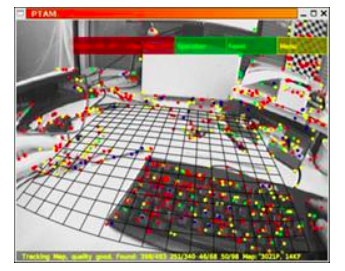
\includegraphics[width=0.7\linewidth]{image/Talk/9.png}  %插入的图,包括JPG,PNG,PDF,EPS等,放在源文件目录下

\end{figure}




2011年,Newcombe 等人提出了单目DTAM 系统[11], 其最显著的特点是能实时恢复场景三维模型(如下图)。基于三维模型,DTAM 既能允许AR应用中的虚拟物体与场景发生物理碰撞,又能保证在特征缺失、图像模糊等情况下稳定地直接跟踪。DTAM采用逆深度(Inverse Depth)[12]方式表达深度。如下图,DTAM将解空间离散为M×N×S 的三维网格,其中M× N为图像分辨率,S为逆深度分辨率,采用直接法构造能量函数进行优化求解。DTAM 对特征缺失、图像模糊有很好的鲁棒性,但由于DTAM 为每个像素都恢复稠密的深度图, 并且采用全局优化,因此计算量很大,即使采用GPU 加速, 模型的扩展效率仍然较低。
\begin{figure}[H]%%图
	\centering  %插入的图片居中表示
	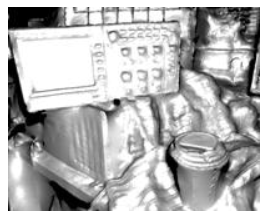
\includegraphics[width=0.7\linewidth]{image/Talk/10.png}  %插入的图,包括JPG,PNG,PDF,EPS等,放在源文件目录下

\end{figure}


2013年,TUM机器视觉组的Engel 等人提出了一套同样也是基于直接法的视觉里程计(visual odometry, VO)系统,该系统2014年扩展为视觉SLAM 系统LSD-SLAM[13],并开源了代码。与DTAM相比,LSD-SLAM 仅恢复半稠密深度图(如下图),且每个像素深度独立计算, 因此能达到很高的计算效率。LSD-SLAM 采用关键帧表达场景,每个关键帧K包含图像 Ik、逆深度图Dk和逆深度的方差Vk。系统假设每个像素x的逆深度值服从高斯分布N(Dk (x),Vk (x))。LSD-SLAM 的前台线程采用直接法计算当前帧t与关键帧k之间相对运动,后台线程对关键帧中每个半稠密抽取的像素点x(梯度显著区域), 在It中沿极线搜索Ik (x)的对应点, 得到新的逆深度观测值及其方差,然后采用EKF更新Dk和Vk 。LSD-SLAM采用位姿图优化来闭合回环和处理大尺度场景。2015年,Engel等人对LSD-SLAM进行了功能拓展,使其能够支持双目相机[14]和全景相机[15]。


\begin{figure}[H]%%图
	\centering  %插入的图片居中表示
	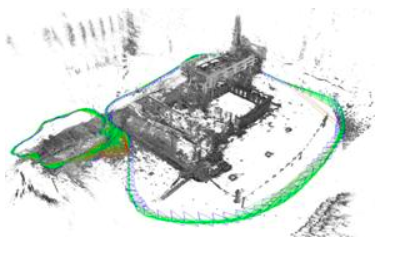
\includegraphics[width=0.7\linewidth]{image/Talk/11.png}  %插入的图,包括JPG,PNG,PDF,EPS等,放在源文件目录下

\end{figure}


2014年,苏黎世大学机器人感知组的Forster等人提出开源的SVO系统[16],该系统对稀疏的特征块使用直接法配准(Sparse Model-based Image Alignment),获取相机位姿,随后根据光度不变假设构造优化方程对预测的特征位置进行优化(Feature Alignment),最后对位姿和结构进行优化(Motion-only BA和Structure-only BA),而在深度估计方面,构造深度滤波器,采用一个特殊的贝叶斯网络[17]对深度进行更新。SVO的一个突出优点就是速度快,由于使用了稀疏的图像块,而且不需要进行特征描述子的计算,因此它可以达到很高的速度(作者在无人机的嵌入式ARM Cortex A9 4核1.6Ghz处理器平台上可以达到55fps的速度),但是SVO缺点也很明显,它没有考虑重定位和闭环,不算是一个完整意义上的SLAM系统,丢失后基本就挂了,而且它的Depth Filter收敛较慢,结果严重地依赖于准确的位姿估计;2016年,Forster对SVO进行改进,形成SVO2.0[18]版本,新的版本做出了很大的改进,增加了边缘的跟踪,并且考虑了IMU的运动先验信息,支持大视场角相机(如鱼眼相机和反射式全景相机)和多相机系统,该系统目前也开源了可执行版本[19];值得一提的是,Foster对VIO的理论也进行了详细的推导,相关的文献[20]成为后续SLAM融合IMU系统的理论指导,如后面的Visual Inertial ORBSLAM等系统。
\begin{figure}[H]%%图
	\centering  %插入的图片居中表示
	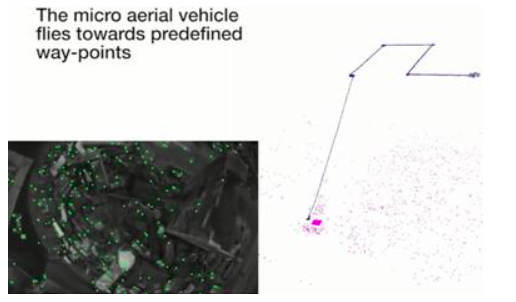
\includegraphics[width=0.7\linewidth]{image/Talk/12.png}  %插入的图,包括JPG,PNG,PDF,EPS等,放在源文件目录下

\end{figure}


2015年,Mur-Artal 等提出了开源的单目ORB-SLAM[21],并于2016年拓展为支持双目和RGBD传感器的ORB-SLAM2[22],它是目前支持传感器最全且性能最好的视觉SLAM系统之一,也是所有在KITTI数据集上提交结果的开源系统中排名最靠前的一个[23]。ORB-SLAM 延续了PTAM 的算法框架,增加了单独的回环检测线程,并对框架中的大部分组件都做了改进,归纳起来主要有以下几点:1)ORB-SLAM追踪、建图、重定位和回环检测各个环节都使用了统一的ORB 特征[24],使得建立的地图可以保存载入重复利用;2)得益于共视图(convisibility graph)的使用,将跟踪和建图操作集中在一个局部互见区域中,使其能够不依赖于整体地图的大小,能够实现大范围场景的实时操作;3)采用统一的BoW词袋模型进行重定位和闭环检测,并且建立索引来提高检测速度;4)改进了PTAM只能手工选择从平面场景初始化的不足,提出基于模型选择的新的自动鲁棒的系统初始化策略,允许从平面或非平面场景可靠地自动初始化。后来,Mur-Artal又将系统进行了拓展,形成了融合IMU信息的Visual Inertial ORB-SLAM[25],采用了Foster的论文[]提出的预积分的方法,对IMU的初始化过程和与视觉信息的联合优化做了阐述。
\begin{figure}[H]%%图
	\centering  %插入的图片居中表示
	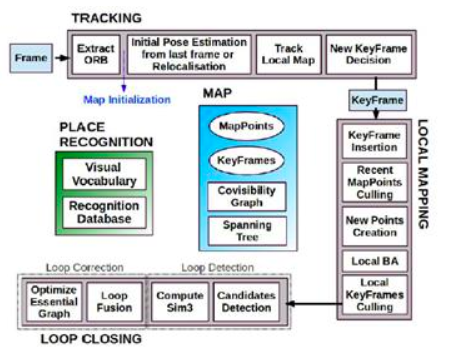
\includegraphics[width=0.7\linewidth]{image/Talk/13.png}  %插入的图,包括JPG,PNG,PDF,EPS等,放在源文件目录下

\end{figure}


2016年,LSD-SLAM的作者,TUM机器视觉组的Engel等人又提出了DSO系统[26]。该系统是一种新的基于直接法和稀疏法的视觉里程计,它将最小化光度误差模型和模型参数联合优化方法相结合。为了满足实时性,不对图像进行光滑处理,而是对整个图像均匀采样。DSO不进行关键点检测和特征描述子计算,而是在整个图像内采样具有强度梯度的像素点,包括白色墙壁上的边缘和强度平滑变化的像素点。而且,DSO提出了完整的光度标定方法,考虑了曝光时间,透镜晕影和非线性响应函数的影响。该系统在TUM monoVO、EuRoC MAV和ICL-NUIM三个数据集上进行了测试,达到了很高的跟踪精度和鲁棒性。
\begin{figure}[H]%%图
	\centering  %插入的图片居中表示
	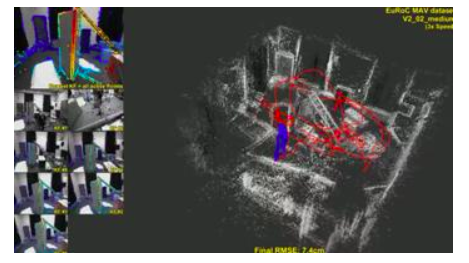
\includegraphics[width=0.7\linewidth]{image/Talk/14.png}  %插入的图,包括JPG,PNG,PDF,EPS等,放在源文件目录下

\end{figure}


2017年,香港科技大学的沈绍劼老师课题组提出了融合IMU和视觉信息的VINS系统[27],同时开源手机和Linux两个版本的代码,这是首个直接开源手机平台代码的视觉IMU融合SLAM系统。这个系统可以运行在iOS设备上,为手机端的增强现实应用提供精确的定位功能,同时该系统也在应用在了无人机控制上,并取得了较好的效果。VINS-Mobile使用滑动窗口优化方法,采用四元数姿态的方式完成视觉和IMU融合,并带有基于BoW的闭环检测模块,累计误差通过全局位姿图得到实时校正。
\begin{figure}[H]%%图
	\centering  %插入的图片居中表示
	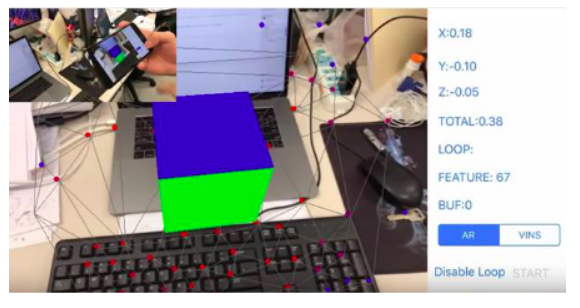
\includegraphics[width=0.7\linewidth]{image/Talk/15.png}  %插入的图,包括JPG,PNG,PDF,EPS等,放在源文件目录下

\end{figure}

\section{漫谈 SLAM 技术(下)}

\subsection{视觉SLAM系统关键问题}

结合上述介绍的SLAM系统,我们从以下几个方面分析视觉SLAM系统需要考虑的关键问题。

(1)图像信息使用

视觉SLAM方法根据使用图像信息的不同可分为直接法,间接法。

直接法,常见于稠密或半稠密的SLAM中,指的是采用图像上每个像素的信息(亮度值)来估计相机位姿;间接法,常用于稀疏的SLAM中,只使用显著的图像部位(即特征)用于位姿估计的计算。

直接法最基本的原理是亮度一致性约束,由于摄像机可以直接测量光的亮度,那么它的优化目标函数是光度误差(如下图),优化变量可以是两幅图像之间的位姿关系,也可以是特征Patch的位置。

\begin{figure}[H]%%图
	\centering  %插入的图片居中表示
	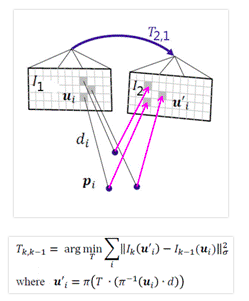
\includegraphics[width=0.7\linewidth]{image/Talk/16.png}  %插入的图,包括JPG,PNG,PDF,EPS等,放在源文件目录下

\end{figure}


根据直接法使用的像素的不同,可以分为稠密直接法和半稠密直接法。在上述介绍的SLAM系统中,DTAM为稠密直接法,它使用了所有的像素;LSD-SLAM和DSO为半稠密直接法,它使用了梯度明显的像素;SVO也为半稠密直接法,它使用了FAST特征点周围邻域的像素。直接方法较多的使用了图像上像素的信息,在纹理较差的部分比间接法更鲁棒。但当场景中的光照变化后,直接法容易失效,亮度一致性约束要求两幅图像之间的光度误差尽可能地小。

间接法使用图像中的特征(点或者线)进行匹配,然后根据匹配关系求解(如下图),它的优化目标函数是特征的重投影误差,优化的变量一般为相对位姿。间接法选取的特征一般要求比较显著,对视角和光照变化具有不变性,对模糊和噪声有一定的弹性,这需要在计算速度和特征质量上取得平衡。计算机视觉领域研究了很多不同的特征提取和特征描述,它们对旋转、尺度不变,和计算速度的性能都不一样。选择合适的特征依赖于平台的计算能力,视觉SLAM算法运行的环境,还有图像的帧率。可选的角点提取器如Harris角点(Harris and Stephens, 1988)、Shi-Tomasi角点(Shi and Tomasi, 1994),FAST角点(Mair et al, 2010)等,特征描述包括但不限于BRIEF,BRISK,SURF,SIFT,FREAK,ORB和像素级别局部区块特征等。
\begin{figure}[H]%%图
	\centering  %插入的图片居中表示
	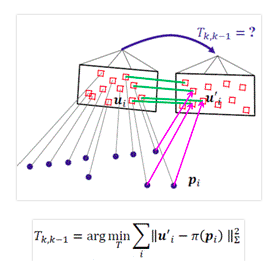
\includegraphics[width=0.7\linewidth]{image/Talk/17.png}  %插入的图,包括JPG,PNG,PDF,EPS等,放在源文件目录下

\end{figure}

使用间接法的SLAM系统一般都是稀疏的,因为它们只使用了图像的很少一部分像素的信息。在上述介绍的SLAM系统中,PTAM、ORBSLAM、VINS都属于间接法的SLAM系统。

(2)数据关联

数据关联就是在不同图像之间建立对应关系,也就是把在多个视角看到的同样的图像部分关联起来,这样才能为后续恢复三维结构做好基础。

特征对应主要有三类:2D-2D,3D-2D和3D-3D。

2D-2D的对应通常用于SLAM系统初始化的时机,这时没有地图,也没有两幅图像之间的相机变换,只能使用2D-2D的数据关联。为了减少计算时间,避免错误数据关联的可能性,可以用第一幅图像的特征2D位置定义一个搜索窗口在第2幅图像中进行搜索,并采用特征描述之间的相似度进行度量。对于像素描述子的局部区块,通常使用模板(patch)匹配中差值的平方和(SSD),或者为了增加对于光照变化的鲁棒性,使用零均值像素灰度差平方和 (ZMSSD),或者零均值归一化交叉相关(ZNCC);对于高层特征描述子,比如ORB,SIFT和SURF,可能会采用L1范数(向量中各个元素绝对值之和,就是绝对值相加,又称曼哈顿距离),L2范数(就是欧几里德距离)或汉明距离,为了加速匹配的搜索过程,可以采用KD树或词袋(BoW)。

3D-2D的特征对应常用于SLAM系统的运行阶段,前一相机位姿估计和场景3D结构已知,需要估计2D特征和这些3D路标在图像中投影的对应关系,有了这个对应关系,就可以通过PnP的方法来求解当前图像和上一帧之间的相对位姿,通常计算PnP时为了排除外点的干扰会结合RANSAC的方法进行。

3D-3D的数据对应主要用来估计和校正回环的累积误差,计算能使回环对齐的相似变换。在RGBD或双目系统中,还可以利用两帧之间的3D结构信息进行三维ICP配准来计算相对位姿,实现三维结构的对齐。

(3)初始化

单目的SLAM系统需要进行初始化,因为单帧图像数据并不能获取深度信息,也不能生成初始的地图。而RGBD和双目的SLAM系统由于单帧图像数据即可获取深度信息,所以不需要进行初始化操作。单目SLAM的初始化,只知道两幅图像之间的关联数据,初始相机位姿和场景结构都是未知的。

早期的MonoSLAM,系统初始化利用一个已知尺寸的平面矩形实现,将相机摆放在该矩形前已知距离的地方,利用平面矩形的四个角点计算初始位姿。

后来的SLAM系统,包括PTAM、SVO、ORBSLAM,都采用如下的流程进行初始化。
\begin{figure}[H]%%图
	\centering  %插入的图片居中表示
	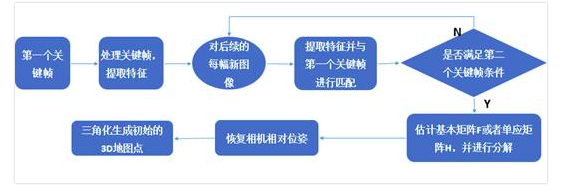
\includegraphics[width=0.7\linewidth]{image/Talk/18.png}  %插入的图,包括JPG,PNG,PDF,EPS等,放在源文件目录下

\end{figure}


PTAM使用单应矩阵初始化,此时场景应该由2D平面组成。PTAM要求用户手工选择前两个关键帧,而且用户在第一个和第二个关键帧之间,需要与场景平行地执行一个缓慢平滑且相对明显的平移运动。PTAM从第1个关键帧提取FAST特征点,在后来的每一帧图像中,采用2D-2D数据关联方法追踪,直到用户插入第2个关键帧。 特征匹配采用ZMSSD,由于没有考虑图像形变,匹配过程对运动模糊和由于相机旋转比较敏感,因此在初始化过程中对用户的运动状态要求比较严格。为了使匹配错误最小化,特征需要在两帧之间对称搜索,如果两个方向的匹配不一致,特征就会被丢弃。第2个关键帧成功加入之后,则采用MLESAC28的方法来计算两个关键帧之间的单应矩阵H,随后利用文献29的方法对H进行分解来恢复相机相对位姿。PTAM初始化非常脆弱,需要技巧去运行,尤其是对于没有经验的用户。另外,当初始化场景不是二维平面,或用户运动状态不恰当的时候,系统退化,容易崩溃。

SVO也使用单应矩阵进行初始化,但SVO不需要用户输入,系统启动时获取第一个关键帧并提取FAST特征,然后用图像间的KLT算法跟踪特征,为了避免用户二次输入,SVO实时检测第一个关键帧和当前图像间的特征点平移量的中值,当这个值达到一定的阈值,算法认为已经获得了足够的视差,开始估计单应矩阵,然后分解单应矩阵并校验相机位姿,得到正确的位姿估计,并三角化对应的内点形成地图点。在第二个图像作为关键帧加入地图管理线程之前,利用捆集调整优化这两个图像帧以及其关联的地图点。与PTAM一样,SVO的初始化同样要求平面场景。

LSD-SLAM的初始化不需要使用两视图几何,它从第1个视角随机初始化场景的深度,然后通过随后的图像不断对场景深度进行修正。图像中梯度明显的像素点的深度被初始化为随机的分布,并赋值为较大的方差后放入系统。第一个初始化的关键帧和后面的图像配准后,跟踪直接开始。图像不断输入,初始特征点的深度测量用滤波方法优化,直到收敛。这种方法不存在两视图几何的退化问题;但在深度收敛之前需要处理大量图像,需要一个中间跟踪过程,生成的地图也不可靠。

在ORB-SLAM中,为了解决上述问题,作者建议并行计算基本矩阵和单应矩阵(用RANSAC方法),并评估两种方法的对称传输误差来选择合适的模型。完成之后,就会进行适当的分解,恢复出相机的位姿,并三角化生成初始地图点,最后通过捆集调整优化地图。如果选择的模型导致跟踪质量差,或者图像上的特征匹配较少,初始化就会迅速被系统丢弃,重新进行初始化,这保证了初始化的可靠性。

(4)位姿估计

因为数据关联计算量巨大,对于每个新图像的位姿,如果能够有个位姿先验,那么对于缩小数据关联的范围就会非常有益。所以,建立这么一个先验是大部分SLAM系统位姿估计的第一个任务。PTAM,ORB SLAM,都在平滑的相机运动状态下采用恒定速度运动模型作为当前图像位姿的先验。但是,在相机运动方向上突然改变时,这样的模型就容易失效。LSD-SLAM和SVO都假设在随后的图像上(这种情况下都是用高帧率相机)相机位姿没有明显改变,因此它们给当前图像位姿和前一个跟踪到的图像分配相同的先验信息。

下图是位姿估计的流程,前一幅图像的位姿用于指导数据关联流程,它可以帮助从当前地图中提取可见的子图,从而减少盲目投影整个地图的计算开销;另外,它还可以为当前图像位姿提供先验,这样特征匹配只在很小的区域内进行搜索,而不是搜索整个图像;最后,它还可以作为优化相机位姿的迭代初值。
\begin{figure}[H]%%图
	\centering  %插入的图片居中表示
	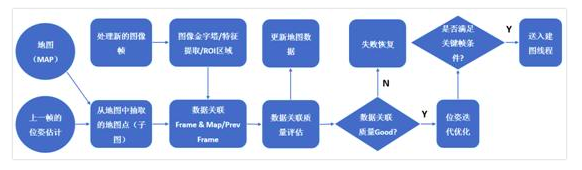
\includegraphics[width=0.7\linewidth]{image/Talk/19.png}  %插入的图,包括JPG,PNG,PDF,EPS等,放在源文件目录下

\end{figure}

下图演示了间接法的相机位姿是如何估计的,Cm是用运动模型估计的新图像位姿,C2是真实的相机位姿。利用Cm,将上一帧可见的地图点重投影到新图像上,在投影点周围一个搜索窗口Sw内进行数据关联,系统使用欧式变换参数(SE3变换)最小化重投影误差d。为了获得对外点(错误匹配的特征)的鲁棒性,目标函数最小化会利用核函数处理掉重投影误差比较大的特征。
\begin{figure}[H]%%图
	\centering  %插入的图片居中表示
	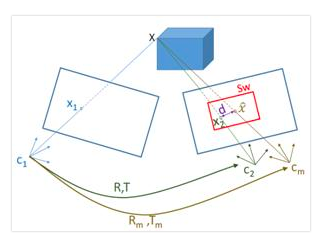
\includegraphics[width=0.7\linewidth]{image/Talk/20.png}  %插入的图,包括JPG,PNG,PDF,EPS等,放在源文件目录下

\end{figure}


(5)地图构建

不同的SLAM系统采用的地图表示形式不同,对于直接法的SLAM系统,由于恢复所有像素或者像素块的三维信息,它们生成地图为稠密或者半稠密的地图;而对于间接法的SLAM系统,它们仅恢复特征点的三维信息,生成的地图为稀疏的地图。无论是稠密、半稠密还是稀疏的地图,都可以看做三维的点云,虽然点云可以存储地图点的位置、特征和法线等,但是它们却不能反映相机位姿之间的关联,所以在SLAM系统中引入了位姿图(Pose Graph),如LSD-SLAM、ORB-SLAM。为了构建位姿图,SLAM系统会从图像帧中挑选一些帧作为关键帧,这些关键帧即为真实场景在不同位姿处的快照。关键帧包含了位姿信息和与地图点云的观测关系,这些关键帧构成了位姿图顶点,它们之间的连接构成了位姿图的边,两个关键帧之间共视的地图点的个数就是这条边的权值。

下图是地图构建的一般流程。可以看到地图构建需要处理两个方面的工作:新的地图元素的加入和已有地图数据的维护。
\begin{figure}[H]%%图
	\centering  %插入的图片居中表示
	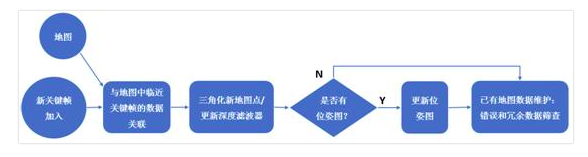
\includegraphics[width=0.7\linewidth]{image/Talk/21.png}  %插入的图,包括JPG,PNG,PDF,EPS等,放在源文件目录下

\end{figure}
新地图元素的加入主要是三维地图点和关键帧。现代的SLAM系统一般都会选取适当的关键帧,以达到场景的精简表示(如PTAM、SVO、LSD-SLAM通过明显的位姿变化原则添加新关键帧,ORB-SLAM通过明显的场景视图变化原则添加新关键帧);在新地图点生成方面,PTAM和ORB-SLAM通过优化关键帧位姿,根据匹配点三角化生成新的地图点,而SVO和LSD-SLAM通过图像帧与关键帧的匹配不断更新深度滤波器,最后利用收敛的特征点的深度来描述新地图点。

已有地图数据的维护主要采用优化的方法对关键帧和地图点位姿进行优化,减少累积误差,并对冗余或错误的关键帧和地图点进行筛除,维护地图数据的有效性和正确性。由于地图数据维护多采用局部BA和全局BA的方法,计算较为耗时,PTAM、LSD-SLAM和ORB-SLAM均单独开辟线程进行处理。

(6)重定位

重定位解决SLAM系统在遭遇突然的剧烈运动或者无特征区域等情况时,跟踪丢失后重新找回的问题。如果不能有效的重定位,SLAM系统前面建立的地图就不能再利用,系统就会失败。

PTAM在检测到跟踪失败后,会将后续每一帧的缩略图SBI(Small Blurry Image)与所有关键帧的SBI进行比较,如果与其灰度的差异小于一定的阈值,那么通过ESM方法估计其相对旋转,然后将地图点投影到当前帧寻找匹配,如果匹配足够,则计算精确位姿,重定位成功。这种方法需要丢失时的位姿与已有关键帧的位姿比较相近才可以成功,在有大的平移时会失败。

SVO简单将图像帧与丢失前最后一次有效位姿附近最近的关键帧进行匹配,如果匹配成功则重定位成功。这种重定位策略对于光照变化和大的平移都很敏感,很容易失败。

LSD-SLAM随机从位姿图中选择一个具有两个以上相邻关键帧的关键帧,并试图将当前帧与它进行匹配,如果外点/内点比率较大,那么丢弃该关键帧,重新随机选择;否则接着测试所有与它相邻的关键帧,如果相邻的关键帧中内点/外点比率较大的关键帧数多于外点/内点比率较大的关键帧数,或者存在多于五个的内点/外点比率较大的关键帧,那么选择内点/外点比率最大的关键帧进行跟踪,重定位成功。

ORB-SLAM的重定位会调用它的位置识别模块,该模块基于BoW进行,它计算当前图像的BoW向量,与地图中所有关键帧的BoW向量比较,找出所有匹配得分高于75%最好低分的关键帧作为候选。对这些候选进行匹配和RANSAC PnP计算,如果内点满足阈值条件,就认为重定位成功。

(7)回环检测

回环检测对于消除SLAM系统长时间运行的漂移有非常重要的作用,如果能够识别到过的地方,那么回环的两端就可以对齐,全局的尺度一致性就能够保证。

LSD-SLAM的做法是每当加入一个新关键帧时,通过FABMAP (Glover et al, 2012)中的Appearance Bbased model搜索与空间最近的10个关键帧的匹配,一旦检测到闭环,则对位姿图进行优化,计算相似变换对齐回环两端,并将回环误差分散到到各个关键帧中。

ORB-SLAM回环检测使用重定位时同样的基于BoW的地点识别模块,它可以为新加入的关键帧从已有关键帧数据库中高效快速的提取回环候选。为了确信回环和排除干扰,它引入连续一致性约束。确信回环之后,同样计算一个相似变换对齐回环两端。然后对关键帧和地图点进行调整,融合重复的地图点,并且执行一个基于位姿图的全局优化。

4. SLAM的实现难点
在《SLAM for Dummy》中,有一句话说的好:“SLAM并不是一种算法,而是一个概念”。(SLAM is more like a concept than a single algorithm.)

SLAM是多个学科多个算法的不同策略组合,它融合了图像处理,几何学,图理论,优化和概率估计等学科的知识,需要扎实的矩阵、微积分、数值计算知识,SLAM跟使用的传感器和硬件平台也有关系,研究者需要具备一定的硬件知识,了解所使用的传感器的硬件特性。所以,根据不同的应用场景,SLAM研究者和工程师必须处理从传感器模型构建到系统集成的各种实践问题。

从上面章节的分析可以看出,SLAM的各个环节用到的技术是偏传统的。与当前大热的深度学习“黑箱模型”不同,SLAM的各个环节基本都是白箱,能够解释得非常清楚。但SLAM却并不是上述各种算法的简单叠加,而是一个系统工程,里面有很多TradeOff。

比如SLAM需要平衡实时性和准确性,SLAM一般是多线程并发执行,资源的分配、读写的协调、地图数据的管理、优化和准确性、关键参数和变量的不确定性以及高速高精度度的姿态跟踪等,都是需要解决的问题。

SLAM还需要考虑硬件的适配,SLAM的数据来源于传感器,有时是多个传感器融合,传感器的质量对SLAM的效果影响很大。例如,如果SLAM使用的相机图像噪点非常多,那么就会对姿态跟踪产生不好的影响,因为特征点提取会很不一致;再比如在VIO系统中,如果相机和IMU的时间戳不一致(至少毫秒级),也会影响算法精度甚至算法失败。多个传感器的分别校准和互相校准,乃至整个系统众多参数的调整,都是非常耗费时间的工程问题。

由于产品和硬件高度差异化,而SLAM相关技术的整合和优化又很复杂,导致算法和软件高度碎片化,所以市场上目前还没有一套通用普适的解决方案,在短时间内也不会有。

5. SLAM的未来
SLAM未来的发展趋势有两大类[]:一是朝轻量级、小型化方向发展,让SLAM能够在嵌入式或手机等小型设备上良好运行,然后考虑以它为底层功能的应用,比如手机端的AR和无人机SLAM等。在这些应用中,我们不希望SLAM占用所有计算资源,所以对SLAM的小型化和轻量化有非常强烈的需求。另一方面则是利用高性能计算设备,实现精密的三维重建、场景理解等功能。在这些应用中,我们的目的是完美地重建场景,而对于计算资源和设备的便携性则没有多大限制,由于可以利用GPU,这个方向和深度学习也有结合点。

(1)多传感器融合SLAM

实际的机器人和硬件设备,通常都不会只携带一种传感器,往往是多种传感器的融合。比如机器人除了视觉传感器,还通常具有激光雷达、里程计、IMU等,手机除了摄像头,也带有IMU、磁力计等传感器。融合多种传感器的信息对于提高SLAM系统的精度和鲁棒性有着重要的意义。比如目前手机上的VIO的研究,它将视觉信息和IMU信息融合,实现了两种传感器的优势互补,为SLAM的小型化与低成本化提供了非常有效解决方案,取得了良好的效果(如苹果ARKit)。

(2)语义SLAM

SLAM的另一个方向就是和深度学习技术结合。到目前为止,SLAM的方案都处于特征点或者像素的层级。关于这些特征点或像素到底来自于什么东西,我们一无所知。这使得计算机视觉中的SLAM与我们人类的做法不怎么相似,至少我们自己从来看不到特征点,也不会去根据特征点判断自身的运动方向。我们看到的是一个个物体,通过左右眼判断它们的远近,然后基于它们在图像当中的运动推测相机的移动。SLAM和语义的结合点主要有两个方面:

语义帮助SLAM。如果有了物体识别的语义信息,就能得到一个带有标签的地图,物体信息可为回环检测、BA优化带来更多的条件。

SLAM帮助语义。物体识别和分割都需要大量的训练数据。要让分类器识别各个角度的物体,需要从不同视角采集该物体的数据,然后进行人工标定,非常辛苦。而SLAM中,由于我们可以估计相机的运动,可以自动地计算物体在图像中的位置,节省人工标定的成本。如果有自动生成的带高质量标注的样本数据,能够很大程度上加速分类器的训练过程。

此外,未来的SLAM技术将会越来越注重算法和硬件的深度结合,专用处理器(如HoloLens HPU)和一体化功能模组(如Tango模组)也是未来的发展方向,这将会大大降低现有硬件平台的计算能力瓶颈和算法调试门槛,带给用户更流畅的体验。

技术发展永无止境,SLAM的未来也才刚刚开始,让我们拭目以待!





\chapter{RGB-D实时重建那些事}

摘录自 http://www.knowsky.com/1053847.html



基于RGB-D的三维重建要从RGB-D相机说起,微软早在2010年就把Kinect折腾出来了,2011年发布了Kinect SDK,2012年发布了可以用来做开发的Kinect版本(可以拿来做学术研究),2011年SIGGRAPH会议上,微软展示了KinectFusion实时重建算法,也就是说做研究的内部人员早就开始拿着Kinect玩了。KinectFusin算法是鼎鼎大名的Newcombe、Davison和微软的部分研究人员提出来的,Newcombe提出单目实时稠密重建算法DTAM [1],RGB-D实时稠密重建KinectFusion算法[2],和动态非刚体(4D)重建DynamicFusion算法 [3],几个工作在小领域都是开山大作。Davison是Newcombe导师,在SLAM领域是开山鼻祖级人物。在RGB-D相机出现之前,采用普通相机很难实现实时稠密重建的(基于高精度结构光可以),也可以说KinectFusion算法首次实现了基于廉价消费类相机的实时刚体重建,把实时三维重建推到可以商业化的地步,也使得实时三维重建这个学科的基础研究,可以支撑得起微软Hololens,Facebook Oculus AR产品的应用需求。关于KinectFusion算法不再多说,前面泡泡有讲,也可以参照博客 [4]。

在学术界,KinectFusion算法一经展示,大家一看,哇,效果这么好,好了,游戏规则变了,人家用深度传感器直接测深度做实时重建,你用普通的单目脱了鞋也追不上,而且这阵势明显离商业化不远了,一块大肥肉来袭。话说KinectFusion算法虽然出的早,框架确实好,也不愧是顶级大牛的工作,2011年以来学术界基于RGB-D刚体重建提出了许多工作,但是基本框架都差不太多,如果看大牛们发表的论文,到2013年,做学术研究的顶级大牛们觉得这块的大块肥肉基本被分割没了,转而开始做动态非刚体重建,2014年斯坦福大牛的工作[5]只能完成变化小的非刚体的重建,2015年Newcombe提出的DynamicFusion算法重建动态非刚体,重建的非刚体只能缓慢变化,2016年出现的Fusion4D算法[7],采用多个深度相机,可以重建快速变化的非刚体,也使得非刚体重建可以达到商业化地步,视频序列可以记录变换着的2维的数据,4D动态非刚体重建可以记录变化着的3维数据!

再把目光投回到刚体重建,话说KinectFusion算法开辟了RGB-D实时重建的时代(只用到深度相机),但是SLAM中每个算法都注定是不完美的,你不完美,我就要完善你,大牛们先把大块的补丁补补。KinectFusion算法用TSDF模型表示重建好的三维场景,TSDF模型也可以参照博客[4],TSDF模型在表示重建的场景时,把场景均匀划分,那我场景大的时候怎么办?采用TSDF模型重建大场景只能增大显存或者缩小网格的密度了,而显存是固定的,网格密度低了重建的精度就差,而且TSDF模型是采用GPU遍历每个网格点进行更新,当分配的网格点多时,更新速度会慢。13年SIGGRAPH出的两篇文章[8-9],解决TSDF模型显存消耗和计算消耗的问题,Voxel Hashing [8] 因为算法开源,而且模型更新速度快,显存耗费资源少,在业内广为人知,牛津大学的工作InfiniTAM [10]也是对[8]的改进(算法开源)。Surfel模型是实时三维重建另一个比较常用的三维表示模型,Srufel模型可以参考ElasticFusion算法[15]或者博客[17]。此外Kintinuous算法[14]采用移动立方体的方式解决显存不足的问题,算法开源,代码写的也是很溜。

KinectFusion采用ICP算法估计两帧之间的位姿,在估计位姿时只用到深度图像,采用点云配准的方式计算两帧之间的位姿变换。ICP算法在匹配两幅点运时,需要赋予初始值,而在实时三维重建中,两帧之间的位姿变换小,新获取帧的位姿用上一帧的位姿初始化。KinectFusion算法和一般SLAM或者VO/VIO算法不同的是,在估算位姿时,将当前帧获取的深度图像和从模型投影获取的深度图像进行配准,这种配准方式被称为frame-to-model,具体可以参见KinectFusion论文和KinectFusion博客,采用frame-to-model的方式配准,比传统意义上的SLAM算法位姿估计和模型重建都更加准确,具体参见KinectFusion论文。而且这种frame-to-model的方式在近年提出的基于RGB-D的重建算法中被广泛采用(在论文里成为标准化的算法)。既然说到SLAM,这里阐述下实时三维重建和SLAM的异同(个人观点),一般意义下的SLAM//VO/VIO算法(PTAM、ORB-SLAM、DVO-SLAM、LSD、DSO、SVO、OKVIS、ROVIO)注重位姿估计,建图效果不好或者没有建图,而RGB-D实时重建除了注重位姿估计,还注重建建图。上述列举的SLAM/VO/VIO算法,在估计位位姿时,只利用CPU,而当前实时三维重建中,基于GPU的frame-to-mode形式的RGB-D直接法[11-13]和ICP算法成为位姿估计的标配方法,TSDF模型更新也通常通过GPU实现,Surfel模型更新通常通过OpenGL实现。

说完实时重建位姿估计和三维模型表示,再说下回环。VO/VIO没有回环检测和回环优化,算法跑的时间越长,累积误差越大。SLAM里通常通过回环检测和回环优化来减小累积误差(在扫描的时候,扫描的轨迹形成不了闭环也不可以)。ORB-SLAM在处理闭环时,在global BA优化完成后,还需要将优化前后的特征融合,因为回环前后,同一个区域的特征会被初始化两次,如果没有融合,会造成场景中同一个特征点在地图中多次出现。同理,在实时重建中,如果扫描返回到之前重建过的区域,同一个场景会被重建两次,而位姿轨迹通常是带有误差的,同一个场景两次重建的结果会错开。RGB-D实时重建通常不考虑回环,不做回环检测和回环优化(KinectFusion、Voxel Hashing和InfiniTAM等),尽管RGB-D实时重建采用frame-to-model的形式做位姿估计,比frame-to-frame的形式更加准确,位姿估计不可避免也会有累计误差,没有回环的实时重建算法跑的时间长,或者相机运动轨迹长时,重建的三维场景也会越来越不靠谱,如果考虑回环,回环检测和回环优化和一般意义上的SLAM算法相差不大(特征点基于BA、或者优化pose-graph),但是回环优化好之后怎么更新重建的地图?好了,问题来了,Thomas Whelan的两个工作Kintinuous [14]和ElasticFusion [15]有处理回环,方法是采用embedded deformation graph对齐回环处重建的点云,算法可以参考论文,也可以参考博客[16-17],此外斯坦福大学的工作BundleFusion [18]也有处理回环。个人认为不处理回环的实时重建算法适合做AR,而处理回环的时候,回环检测和回环处重建地图的对齐都不好处理,当前回环检测算法不够鲁棒,回环处地图对齐Kintinuous算法效果并不好(也可能只是开源代码处理的不好,作者有可以处理的好的方法),BundleFusion算法现在还未开源,很值得期待开源。

欢迎做实时重建/SLAM/VIO/VO的小伙伴多多指教。

[1] Newcombe R A, Lovegrove S J, Davison A J. DTAM: Dense tracking and mapping in real-time[C]//Computer Vision (ICCV), 2011 IEEE International Conference on. IEEE, 2011: 2320-2327. 

[2] Newcombe R A, Izadi S, Hilliges O, et al. KinectFusion: Real-time dense surface mapping and tracking[C]//Mixed and augmented reality (ISMAR), 2011 10th IEEE international symposium on. IEEE, 2011: 127-136. 

[3] Newcombe R A, Fox D, Seitz S M. Dynamicfusion: Reconstruction and tracking of non-rigid scenes in real-time[C]//PRoceedings of the IEEE conference on computer vision and pattern recognition. 2015: 343-352. 

[4] http://blog.csdn.net/fuxingyin/article/details/51417822 

[5] Zollhöfer M, Nießner M, Izadi S, et al. Real-time non-rigid reconstruction using an RGB-D camera[J]. ACM Transactions on Graphics (TOG), 2014, 33(4): 156. 

[6] Dou M, Khamis S, Degtyarev Y, et al. Fusion4d: Real-time performance capture of challenging scenes[J]. ACM Transactions on Graphics (TOG), 2016, 35(4): 114. 

[7] Dou M, Khamis S, Degtyarev Y, et al. Fusion4d: Real-time performance capture of challenging scenes[J]. ACM Transactions on Graphics (TOG), 2016, 35(4): 114. 

[8] Nießner M, Zollhöfer M, Izadi S, et al. Real-time 3D reconstruction at scale using voxel hashing[J]. ACM Transactions on Graphics (TOG), 2013, 32(6): 169. 

[9] Chen J, Bautembach D, Izadi S. Scalable real-time volumetric surface reconstruction[J]. ACM Transactions on Graphics (TOG), 2013, 32(4): 113. 

[10] Kahler O, Adrian Prisacariu V, Yuheng Ren C, et al. Very high frame rate volumetric integration of depth images on mobile devices[J]. IEEE Transactions on Visualization and Computer Graphics, 2015, 21(11): 1241-1250. 

[11] Steinbrücker F, Sturm J, Cremers D. Real-time visual odometry from dense RGB-D images[C]//Computer Vision Workshops (ICCV Workshops), 2011 IEEE International Conference on. IEEE, 2011: 719-722. 

[12] Whelan T, Johannsson H, Kaess M, et al. Robust real-time visual odometry for dense RGB-D mapping[C]//Robotics and Automation (ICRA), 2013 IEEE International Conference on. IEEE, 2013: 5724-5731. 

[13] Kerl C, Sturm J, Cremers D. Robust odometry estimation for RGB-D cameras[C]//Robotics and Automation (ICRA), 2013 IEEE International Conference on. IEEE, 2013: 3748-3754. 

[14] Whelan T, Kaess M, Johannsson H, et al. Real-time large-scale dense RGB-D SLAM with volumetric fusion[J]. The International Journal of Robotics Research, 2015, 34(4-5): 598-626. 

[15] Whelan T, Leutenegger S, Salas-Moreno R F, et al. ElasticFusion: Dense SLAM Without A Pose Graph[C]//Robotics: science and systems. 2015, 11. 

[16] http://blog.csdn.net/fuxingyin/article/details/51647750 

[17] http://blog.csdn.net/fuxingyin/article/details/51433793 

[18] http://blog.csdn.net/fuxingyin/article/details/52921958 

[19] http://blog.csdn.net/fuxingyin





\nocite{EINAV2010,Havrylchyk2018} 

\bibliographystyle{aer}
\bibliography{reference}




\appendix

\chapter{最优化}\label{附录A}

\section{最小二乘法}
线性最小二乘法的公式如下:

\begin{equation}
	\min_{x}\|Ax-b\|
\end{equation}

其中$Ax$是变量$x$的线性函数。


非线性最小二乘的公式如下:
\begin{equation}
	\min_{x} \|f(x)\|
\end{equation}
其中$f(x)$是变量$x$的非线性函数。


\subsection{线性最小二乘法}

其解为下列方程的解为:
\begin{equation}
A^TAx = A^Tb
\end{equation}
也即
\begin{equation}
x = (A^TA)^{-1}A^Tb
\end{equation}



\subsection{非线性最小二乘法}\label{appendix:non-linear-least-square}
求解非线性最小二乘问题,就是将其变分线性最小二乘来求解,简单来说就是对函数$f(x)$进行线性展开。
\begin{equation}
	f(x) = f(x_n) + J_n(x - x_n) = f(x_n) + J_n\delta x
\end{equation}
\begin{equation}
	\min_{x}\|f(x)\| = \min_{x}\|J_n\delta x - (-f(x_n))\|
\end{equation}

现在非线性最小二乘就变成了线性最小二乘问题,仿照线性最小二乘的解法,得到:
\begin{equation}
	J^TJ\delta x = -J^Tf(x_n)
\end{equation}
也即
\begin{equation}
	\delta x = -(J^TJ)^{-1}J^Tf(x_n)
\end{equation}


\subsection{加权最小二乘}






\end{document}
